\documentclass[11pt]{article}
\usepackage{amssymb, amsthm, amsmath}
\usepackage{bm}
\usepackage{graphicx}
\usepackage[authoryear]{natbib}
\usepackage{bm}
\usepackage{verbatim}
\usepackage{lineno}
\usepackage{times}
\usepackage{soul}
\usepackage{color}
\usepackage{enumitem}
\usepackage{multirow}
\usepackage{setspace}
\usepackage{times}
\usepackage{changepage}
\usepackage{booktabs}
\usepackage{url}
\usepackage{pdflscape}
\usepackage{subfig}

\usepackage[left=1in,top=1in,right=1in]{geometry}
\pdfpageheight 11in
\pdfpagewidth 8.5in
\linespread{2.0}
\newcommand{\btheta}{ \mbox{\boldmath $\theta$}}
\newcommand{\bmu}{ \mbox{\boldmath $\mu$}}
\newcommand{\balpha}{ \mbox{\boldmath $\alpha$}}
\newcommand{\bbeta}{ \mbox{\boldmath $\beta$}}
\newcommand{\bdelta}{ \mbox{\boldmath $\delta$}}
\newcommand{\blambda}{ \mbox{\boldmath $\lambda$}}
\newcommand{\bgamma}{ \mbox{\boldmath $\gamma$}}
\newcommand{\brho}{ \mbox{\boldmath $\rho$}}
\newcommand{\bpsi}{ \mbox{\boldmath $\psi$}}
\newcommand{\bepsilon}{ \mbox{\boldmath $\epsilon$}}
\newcommand{\bomega}{ \mbox{\boldmath $\omega$}}
\newcommand{\bOmega}{ \mbox{\boldmath $\Omega$}}
\newcommand{\bDelta}{ \mbox{\boldmath $\Delta$}}
\newcommand{\bSigma}{ \mbox{\boldmath $\Sigma$}}
\newcommand{\bPsi}{\mbox{\boldmath $\Psi$}}
\newcommand{\bOne}{\mbox{\boldmath $1$}}
\newcommand{\omu}{\overline{\mu}}
\newcommand{\oSigma}{\overline{\Sigma}}
\newcommand{\Yt}{{\tilde Y}}
\newcommand{\bA}{ \mbox{\bf A}}
\newcommand{\bP}{ \mbox{\bf P}}
\newcommand{\bx}{ \mbox{\bf x}}
\newcommand{\bX}{ \mbox{\bf X}}
\newcommand{\bB}{ \mbox{\bf B}}
\newcommand{\bZ}{ \mbox{\bf Z}}
\newcommand{\by}{ \mbox{\bf y}}
\newcommand{\bY}{ \mbox{\bf Y}}
\newcommand{\bz}{ \mbox{\bf z}}
\newcommand{\bh}{ \mbox{\bf h}}
\renewcommand{\bm}{ \mbox{\bf m}}
\newcommand{\br}{ \mbox{\bf r}}
\newcommand{\bt}{ \mbox{\bf t}}
\newcommand{\bs}{ \mbox{\bf s}}
\newcommand{\bb}{ \mbox{\bf b}}
\newcommand{\bL}{ \mbox{\bf L}}
\newcommand{\bu}{ \mbox{\bf u}}
\newcommand{\bv}{ \mbox{\bf v}}
\newcommand{\bV}{ \mbox{\bf V}}
\newcommand{\bW}{ \mbox{\bf W}}
\newcommand{\bG}{ \mbox{\bf G}}
\newcommand{\bH}{ \mbox{\bf H}}
\newcommand{\bw}{ \mbox{\bf w}}
\newcommand{\bo}{ \mbox{\bf o}}
\newcommand{\bfe}{ \mbox{\bf e}}
\newcommand{\iid}{\stackrel{iid}{\sim}}
\newcommand{\ind}{\stackrel{ind}{\sim}}
\newcommand{\dd}{\; \text{d} }
\newcommand{\ddd}{\text{d} }
\newcommand{\indep}{\stackrel{indep}{\sim}}
\newcommand{\converged}{\stackrel{d}{\rightarrow}}
\newcommand{\calR}{{\cal R}}
\newcommand{\calG}{{\cal G}}
\newcommand{\calD}{{\cal D}}
\newcommand{\calS}{{\cal S}}
\newcommand{\calB}{{\cal B}}
\newcommand{\calA}{{\cal A}}
\newcommand{\calT}{{\cal T}}
\newcommand{\calO}{{\cal O}}
\newcommand{\argmax}{{\mathop{\rm arg\, max}}}
\newcommand{\argmin}{{\mathop{\rm arg\, min}}}
\newcommand{\Frechet}{\mbox{Fr$\acute{\mbox{e}}$chet }}
\newcommand{\Matern}{\mbox{Mat$\acute{\mbox{e}}$rn }}
\newcommand{\ballunion}{B_a(\bs_1) \cup B_b(\bs_2) }

\newcommand{\beq}{ \begin{equation}}
\newcommand{\eeq}{ \end{equation}}
\newcommand{\beqn}{ \begin{eqnarray}}
\newcommand{\eeqn}{ \end{eqnarray}}

\newcommand*\patchAmsMathEnvironmentForLineno[1]{%
  \expandafter\let\csname old#1\expandafter\endcsname\csname #1\endcsname
  \expandafter\let\csname oldend#1\expandafter\endcsname\csname end#1\endcsname
  \renewenvironment{#1}%
     {\linenomath\csname old#1\endcsname}%
     {\csname oldend#1\endcsname\endlinenomath}}%
\newcommand*\patchBothAmsMathEnvironmentsForLineno[1]{%
  \patchAmsMathEnvironmentForLineno{#1}%
  \patchAmsMathEnvironmentForLineno{#1*}}%
\AtBeginDocument{%
\patchBothAmsMathEnvironmentsForLineno{equation}%
\patchBothAmsMathEnvironmentsForLineno{align}%
\patchBothAmsMathEnvironmentsForLineno{flalign}%
\patchBothAmsMathEnvironmentsForLineno{alignat}%
\patchBothAmsMathEnvironmentsForLineno{gather}%
\patchBothAmsMathEnvironmentsForLineno{multline}%
}



%184: I'd make this line a little less pessimistic and say "The results of the real data analysis mirror those of the simulation study."
%
%201: Again, less pessimistic: "is that the spatial probit model is suffient for binary data expcept in the most extreme cases with occuring for less than 1% of the observations."  I'd also add here that probit and GEV both outperformed the logit.  Logit is the most common method, so this is news.
%
%
%212: Use %rarity instead of K in case they've forgotten K by now.

\begin{document}\linenumbers

\begin{center}
{\Large {\bf A spatial model for rare binary events}}\\
\today
\end{center}

\section{Introduction}\label{rbs:intro}

The goals of spatial binary data analysis are often to estimate covariate effects while accounting for spatial dependence and to make predictions at locations without samples.
A common approach to incorporate spatial dependence in the model for binary data is relating a continuous spatial process $Z(\bs) \in \mathbb{R}$ to the binary response $Y(\bs)$ by thresholding, $Y(\bs) = I[Z(\bs) > c]$, where $I[\cdot]$ is an indicator function.
In many spatial analyses of binary data, a Gaussian process is used to model $Z(\bs)$.
This is true for both spatial probit and spatial logistic regression.
In this model, spatial dependence is determined by the joint probability that two sites simultaneously exceed the threshold $c$.
However, when $c$ is large, and thus $Y(\bs) = 1$ is rare, then the asymptotic theory suggests that the Gaussian process will model dependence poorly.
In fact, even under strong spatial correlation for $Z$, it gives asymptotic independence \citep{Sibuya1960}, suggesting that for rare binary data, the Gaussian model will not perform very well.

We propose using a latent max-stable process \citep{deHaan1984} for $Z(\bs)$ because it allows for asymptotic dependence.
The max-stable process arises as the limit of the location-wise maximum of infinitely many spatial processes, and any finite-dimensional representation of a max-stable process has generalized extreme value distribution (GEV) marginal distributions.
Max-stable processes are extremely flexible, but are often challenging to work with in high dimensions \citep{Wadsworth2014,Thibaud2013a}.
To address this challenge, methods have been proposed that implement composite likelihood techniques for max-stable processes \citep{Padoan2010,Genton2011,Huser2014}.
Composite likelihoods have been used to model binary spatial data \citep{Heagerty1998}, but not using max-stable processes.
As an alternative to these composite approaches, \citet{Reich2012} present a hierarchical model that implements a low-rank representation for a max-stable process.
We chose to use this low-rank representation for our rare binary spatial regression model.
Our model builds on related work by \citet{Wang2010} who use a GEV link for non-spatial binary data.
The proposed model generalizes this to have spatial dependence.

The paper proceeds as follows.
In \sref{rbs:maxstab} we present the proposed latent max-stable process for rare binary data analysis.
In \sref{rbs:multivariate} we give the bivariate distribution for our model.
In \sref{rbs:spatdep} we show a link between a commonly used measure of dependence between binary variables and another metric for extremal dependence.
The computing for our model is outlined in \sref{rbs:comp}.
Finally, we present a simulation study in \sref{rbs:sim} followed in \sref{rbs:dataanalysis} by a data analysis of two species: \tamarix{} and \hedysarum{} in .
Lastly, in \sref{rbs:conclusions} we provide some discussion and possibilities for future research.

\section{Spatial dependence for binary regression} \label{rbs:maxstab}

Let $Y(\bs)$ be the binary response at spatial location $\bs$ in a spatial domain of interest $\calD \in \mathbb{R}^2$.
We assume $Y(\bs) = I[Z(\bs) > 0]$ where $Z(\bs)$ is a latent continuous max-stable process.
The marginal distribution of $Z(\bs)$ at site $\bs$ is GEV with location $\bX(\bs)^\top \bbeta$, scale $\sigma > 0$, and shape $\xi$, where $\bX(\bs)$ is a $p$-vector of spatial covariates at site $\bs$ and $\bbeta$ is a $p$-vector of regression coefficients.
We set $\sigma = 1$ for identifiability because only the sign and not the scale of $Z$ affects $Y$.
If $\bX(\bs)^\top \bbeta = \mu$ for all $\bs$, then $P(Y = 1)$ is the same for all observations, and the two parameters $\mu$ and $\xi$ are not individually identifiable, so when there are no covariates, we fix $\xi = 0$.
Although $\bbeta$ and $\xi$ could be permitted to vary across space, we assume that they are constant across $\calD$.
At spatial location $\bs$, the marginal distribution (over $Z(\bs)$) is \mbox{$P[Y(\bs) = 1] = 1 - \exp\left[ -\displaystyle\frac{ 1 }{ z(\bs)} \right]$} where $z(\bs) = \left[1 - \xi \bX(\bs)^\top \bbeta\right]^{1 / \xi}$.
This is the same as the marginal distribution given by \citet{Wang2010}.

For a finite collection of locations $\bs_1, \ldots, \bs_n,$ we denote by $\bY = [Y(\bs_1), \ldots, Y(\bs_n)]^T$ the vector of observations.
The spatial dependence of $\bY$ is determined by the joint distribution of the latent variable $\bZ = [Z(\bs_1),\ldots, Z(\bs_n)]^T$.
To incorporate spatial dependence, we consider the hierarchical representation of the max-stable process proposed in \citet{Reich2012}.
Consider a set of positive stable random effect $A_1, \ldots, A_L \iid \text{PS}(\alpha)$ associated with spatial knots $\bv_1, \ldots, \bv_L \in \mathbb{R}^2$.
The hierarchical model is given by
\begin{align} \label{rbeq:hiermodel}
  \bZ(\bs_i) | A_1, \ldots, A_L \ind \text{GEV}[\bX(\bs_i)^\top \bbeta + \theta(\bs_i), \alpha \theta(\bs_i), \xi \alpha] \quad \text{and} \quad \theta(\bs_i) = \left[\sum_{l = 1}^L A_l w_l (\bs_i)^{1 / \alpha} \right]^\alpha
\end{align}
where $w_{l}(\bs_i) > 0$ are a set of $L$ weight functions that vary smoothly across space and satisfy $\displaystyle \sum_{l = 1}^L w_l(\bs) = 1$ for all $\bs$, and $\alpha\in(0,1)$ determines the strength of dependence, with $\alpha$ near zero giving strong dependence and $\alpha=1$ giving joint independence.

Because the latent $\bZ(\bs)$ are independent given the random effects $\theta(\bs)$, the binary responses are also conditionally independent.
This leads to the tractable likelihood
\begin{align} \label{rbeq:condlike}
  Y(\bs_i) | A_l, \ldots, A_L &\ind \text{Bern}[\pi(\bs_i)]
\end{align}
where
\begin{align} \label{rbeq:pyeq1cond}
  \pi(\bs_i) &= 1 - \exp \left\{ -\displaystyle \sum_{ l = 1 }^{L} A_l \left( \frac{ w_{l}(\bs_i) }{ z(\bs_i) } \right)^{ 1/\alpha} \right\}
\end{align}
and $z(\bs) = [1 + \xi \bX(\bs)^\top \bbeta)]^{1 / \xi}$.
Marginally over the $A_l$, this gives
\begin{align}
  Z(\bs) \sim \text{GEV}\left[\bX(\bs)^\top \bbeta, 1, \xi\right],
\end{align}
and thus $P[Y(\bs) = 1] = 1 - \exp\left\{-\displaystyle \frac{1}{z(\bs)}\right\}$.

Many weight functions are possible, but the weights must be constrained so that $\displaystyle \sum_{l=1}^L w_{l}(\bs_i)=1$ for $i=1,\ldots,n$ to preserve the marginal GEV distribution.
For example, \cite{Reich2012} take the weights to be scaled Gaussian kernels with knots $\bv_l$,
\begin{align}\label{rbeq:w}
   w_{l}(\bs_i) = \frac{\exp\left[-0.5\left(||\bs_i-\bv_l||/\rho\right)^2\right]}
                 {\displaystyle \sum_{j=1}^L\exp\left[-0.5\left(||\bs_i-\bv_j||/\rho\right)^2\right]}
\end{align}
where $||\bs_i - \bv_l||$ is the distance between site $\bs_i$ and knot $\bv_l$, and the kernel bandwidth $\rho>0$ determines the spatial range of the dependence, with large $\rho$ giving long-range dependence and vice versa.

After marginalizing out the positive stable random effects, the joint distribution of $\bZ$ is
\begin{align}\label{rbeq:jointCDF}
  G(\bz) = P\left[Z(\bs_1) < z(\bs_1), \ldots, Z(\bs_n) < z(\bs_n)\right] = \exp\left\{-\sum_{l=1}^L\left[\sum_{i=1}^n\left(\frac{w_{l}(\bs_i)}{z(\bs_i)}\right)^{1/\alpha}\right]^{\alpha}\right\},
\end{align}
where $G(\cdot)$ is the CDF of a multivariate GEV distribution.
This is a special case of the multivariate GEV distribution with asymmetric Laplace dependence function \citep{Tawn1990}.

\section{Joint distribution}\label{rbs:multivariate}

We give an exact expression in the case where there are only two spatial locations which is useful for constructing a pairwise composite likelihood \citep{Padoan2010} and studying spatial dependence.
When $n = 2$, the probability mass function is given by
\begin{align} \label{rbeq:biv}
  \text{P}[Y(\bs_i) = y_i, Y(\bs_j) = y_j] = \begin{cases}
    \varphi(\bz), &y_i = 0, y_j = 0\\
    \exp\left\{ - \displaystyle \frac{ 1 }{ z(\bs_i) } \right\} - \varphi(\bz), &y_i = 1, y_j = 0 \\
    \exp\left\{ - \displaystyle \frac{ 1 }{ z(\bs_j) } \right\} - \varphi(\bz), &y_i = 0, y_j = 1 \\
    1 - \exp\left\{ - \displaystyle\frac{ 1 }{ z(\bs_i) } \right\} - \exp \left\{ -\displaystyle \frac{ 1 }{z(\bs_j)} \right\} + \varphi(\bz), \quad &y_i = 1, y_j = 1
  \end{cases}
\end{align}
where $\varphi(\bz) = \exp \left\{ - \displaystyle \sum_{ l = 1 }^{ L } \left[ \left( \displaystyle \frac{ w_{ l }(\bs_i) }{ z(\bs_i) } \right)^{1/\alpha} + \left( \displaystyle \frac{ w_{l }(\bs_j)}{z(\bs_j)} \right)^{1/\alpha} \right]^{\alpha} \right\}$.
For more than two locations, we are also able to compute the exact likelihood when the $n$ is large but the number of events $K = \displaystyle \sum_{i = 1}^n Y(\bs_i)$ is small, as might be expected for very rare events, see \aref{rba:likelihoodderivation}.

 % - Assume Z1 and Z2 are both GEV(\beta,1,1) so that the probability of Yi=1 decreases to zero as beta increases
 % - A common measure of dependence between binary variables is Cohen’s Kappa, K(beta) =
 % - For the spatial model we get K(beta)=
 % - To measure extremal dependence let beta go to infinity so that event are increasing more rare
 % - K = limK(beta) = …
 % - This is similar to the extremal coefficient in Reich and Shaby

\section{Quantifying spatial dependence} \label{rbs:spatdep}

Assume that $Z_1$ and $Z_2$ are both GEV$(\beta, 1, 1)$ so that $P(Y_i = 1)$ decreases to zero as $\beta$ increases.
A common measure of dependence between binary variables is Cohen's Kappa \citep{Cohen1960},
\begin{align}
  \kappa(\beta) = \frac{P_A - P_E}{1 - P_E}
\end{align}
where $P_A$ is the joint probability of agreement $P(Y_1 = Y_2)$ and $P_E$ is the joint probability of agreement under an assumption of independence $P(Y_i = 1)^2 + P(Y_i = 0)^2$.
For the spatial model,
\begin{align*}
  P_A(\beta) &= 1 - 2 \exp\left\{ -\frac{1}{\beta} \right\} + 2 \exp\left\{-\frac{\vartheta(\bs_1, \bs_2)}{\beta}  \right\} \nonumber \\
  P_E(\beta) &= 1 - 2 \exp \left\{ -\frac{1}{\beta} \right\} + 2 \exp \left\{ -\frac{2}{\beta} \right\}, \nonumber
\end{align*}
and
\begin{align} \label{rbeq:kappa}
  \kappa(\beta) &= \frac{P_A(\beta) - P_E(\beta)}{1 - P_E(\beta)} = \frac{\exp\left\{-\displaystyle\frac{\vartheta(\bs_1, \bs_2) - 1}{\beta}  \right\} - \exp \left\{ -\frac{1}{\beta} \right\}}{1 - \exp \left\{ -\frac{1}{\beta} \right\}}
\end{align}
where $\vartheta (\bs_i, \bs_j) = \displaystyle \sum_{ l = 1 }^{ L } \left[ w_{l}(\bs_i)^{ 1/\alpha } +  w_{ l}(\bs_j)^{ 1/\alpha } \right]^\alpha$ is the pairwise extremal coefficient given by \citet{Reich2012}.
To measure extremal dependence, let $\beta \rightarrow \infty$ so that events are increasingly rare.
Then,
\begin{align}
  \kappa = \lim_{\beta \rightarrow \infty} \kappa(\beta) = 2 - \vartheta(\bs_1, \bs_2)
\end{align}
which is the same as the $\chi$ statistic of \citet{Coles2001}, a commonly used measure of extremal dependence.

\section{Computation}\label{rbs:comp}

For small $K$, we can evaluate the likelihood directly.
When $K$ is large, we use Markov chain Monte Carlo (MCMC) methods with the random effects model to explore the posterior distribution.
To overcome challenges with evaluating the positive stable density, we follow \citet{Reich2012} and introduce a set of auxiliary variables $B_1, \ldots, B_L$ following the auxiliary variable technique of \citet{Stephenson2009} (for more details, see Appendix A.3 of \citet{Reich2012}).
So, the hierarchical model is given by
\begin{align}
  Y(\bs_i) | \pi(\bs_i) &\ind \text{Bern}[\pi(\bs_i)] \\
    \pi(\bs_i) &= 1 - \exp \left\{ -\displaystyle \sum_{ l = 1 }^{L} A_l \left( \frac{ w_{l}(\bs_i) }{ z(\bs_i) } \right)^{ 1/\alpha} \right\} \nonumber\\
    % Z(\bs_i) | A_l, \ldots, A_L &\ind \text{GEV}[\bX(\bs_i)^\top \bbeta + \theta(\bs_i), \alpha \theta(\bs_i), \xi \alpha] \nonumber\\
    A_l &\sim \text{PS}(\alpha) \nonumber
\end{align}
with priors $\bbeta \sim \text{N}(\bZero, \sigma^2_\beta \bI_p )$, $\xi \sim \text{N}(0, \sigma^2_\xi)$, $\rho \sim \text{Unif}(\rho_l, \rho_u)$, and $\alpha \sim \text{Beta}(a_\alpha, b_\alpha)$.
The model parameters are updated using Metropolis Hastings (MH) update steps, and the random effects $A_1, \ldots, A_L$, and auxiliary variables $B_1, \ldots, B_L$ are updated using Hamiltonian Monte Carlo (HMC) update steps.
The code for this is available online through \url{https://github.com/sammorris81/rare-binary}.

\section{Simulation study}\label{rbs:sim}

For our simulation study, we generate $n_m = 50$ datasets under 12 different simulation settings to explore the impact of sample size, sampling technique, and misspecification of link function.
We generate data assuming three possible types of underlying process.
For each of the underlying processes, we generate complete datasets on a $100 \times 100$ rectangular grid of $n = 10,000$ locations.
If a simulated population is generated with $K < 50$, it is discarded and a new simulated population is generated.
This is done to guarantee that datasets have no less than $0.5\%$ rarity.
For model fitting, we select a subsample and use the remaining sites to evaluate predictive performance.
For all models, we run the MCMC sampler for 25,000 iterations with a burn-in period of 20,000 iterations.
Convergence is assessed through visual inspection of traceplots.

\subsection{Latent processes} \label{rbs:simsettings}

The first process is a latent max-stable process that uses the GEV link described in \eref{rbeq:hiermodel} with knots on a $50 \times 50$ regularly spaced grid on $[0, 1] \times [0, 1]$.
For this process, we set $\alpha = 0.35$, $\rho = 0.1$, and $\beta_0 \approx 2.97$ which gives $K = 500$ (5\% rarity), on average.
Because there are no covariates, we set $\xi = 0$.
We then set $Y(\bs) = I[Z(\bs) > 0]$.

For the second process, we generate a latent variable from a spatial Gaussian process with a mean of $\text{logit}(0.05) \approx -2.94$ and an exponential covariance given by
\begin{align}
  \text{Cov}(\bs_1, \bs_2) = \tau_\text{Gau}^2 \exp\left\{- \frac{||\bs_1 - \bs_2||}{\rho_\text{Gau}}\right\}
\end{align}
where $\tau_\text{Gau} = 10$ and $\rho_\text{Gau} = 0.1$.
Finally, we generate $Y(\bs_i) \ind \text{Bern}[\pi(\bs_i)]$
where $\pi(\bs_i) = \displaystyle \frac{ \exp\{z(\bs)\}}{1 + \exp\{z(\bs)\} }$.

For the third process, we generate data using a hotspot method.
For this process, we first generate hotspots throughout the space.
Let $n_\text{hs}$ be the number of hotspots in the space.
Then \mbox{$n_\text{hs} - 1 \sim$ Poisson$(2)$}.
This generation scheme ensures that every dataset has at least one hotspot.
We generate the hotspot locations $\bh_1, \ldots, \bh_{n_\text{hs}} \sim$ Unif$(0, 1)^2$.
Let $B_h$ be a circle of radius of radius $r_h$ around hotspot $h = 1, \ldots, n_\text{hs}$.
The $r_h$ differ for each hotspot and are generated i.i.d. from a Unif$(0.03, 0.08)$ distribution.
We set $P[Y(\bs_i) = 1] = 0.85$ for all $\bs_i$ in $B_h$, and $P[Y(\bs_i)] = 0.0005$ for all $\bs_i$ outside of $B_h$.
These settings are selected to give an average of approximately $K = 500$ for the datasets.
\fref{rbfig:simulateddata} gives an example dataset from each of the data settings.

\begin{figure}  % code/analysis/simstudy/combine-tables.R
  \centering
  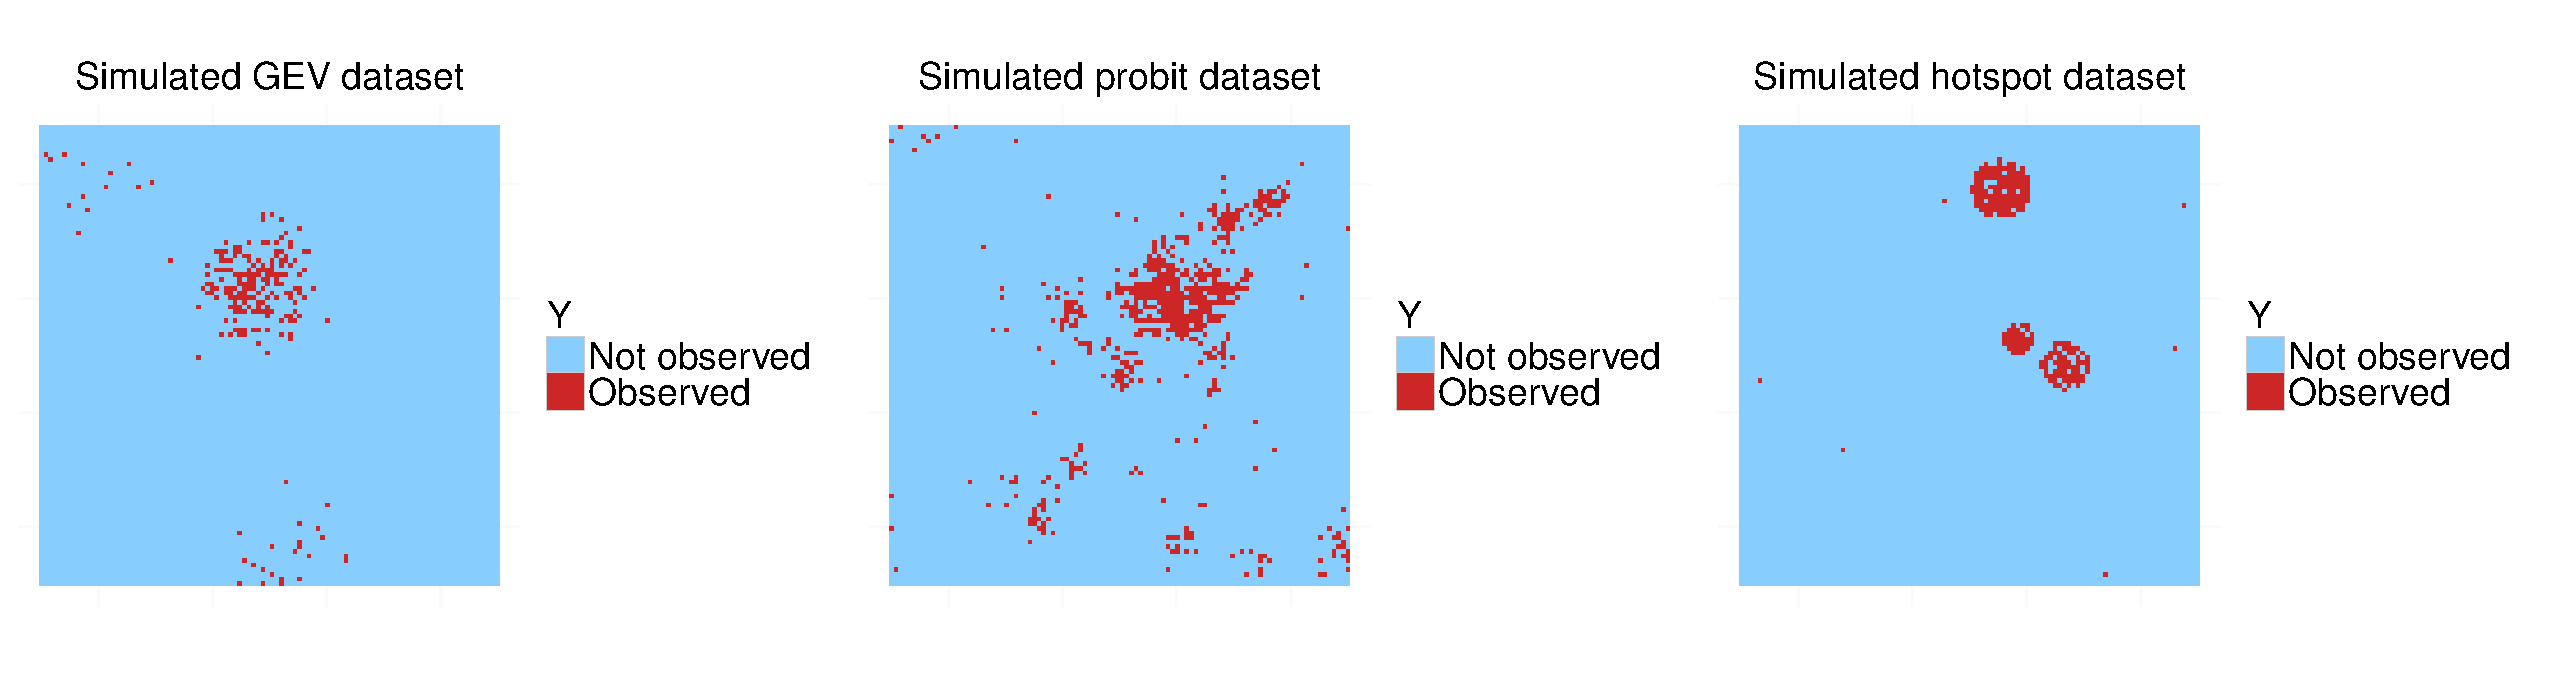
\includegraphics[width=\linewidth, trim={0em, 1em, 0em, 1em}]{plots/simulateddata}
  \caption{One simulated dataset from spatial GEV (left), spatial logistic (center), and hotspot (right) designs.}
  \label{rbfig:simulateddata}
\end{figure}

\subsection{Sampling methods} \label{rbs:simsampling}

We subsample the generated data using $n_s = 100$, $250$ initial locations for two different sampling designs.
The first is a two-stage spatially-adaptive cluster technique (CLU) taken from \citet{Pacifici2016}.
In this design, if an initial location is occupied, we also include the four rook neighbor (north, east, south, and west) sites in the sample.
For the second design, we use a simple random sample (SRS) with the same number of sites included in the cluster sample.
For the GEV setting, when $n_s = 100$, there are on average $117$ sites and at most $142$ sites in a sample, and when $n_s = 250$, there are on average $286$ sites and at most $332$ sites in a sample.
For the logistic setting, when $n_s = 100$, there are on average $118$ sites and at most $147$ sites in a sample, and when $n_s = 250$, there are on average $290$ sites and at most $330$ sites in a sample.
For the hotspot setting, when $n_s = 100$, there are on average $110$ sites and at most $128$ sites in a sample, and when $n_s = 250$, there are on average $275$ sites and at most $306$ sites in a sample.

\subsection{Methods} \label{rbs:methods}

For each dataset, we fit the model using three different models: the proposed spatial GEV model, a spatial probit model, and a spatial logistic model.
Logistic and probit methods assume the underlying process is Gaussian.
In this case, we assume that $Z(\bs)$ follows a Gaussian process with mean $\bX(s)^\top \bbeta$ and unit variance.
For the simulation study, we use an intercept only model.
The marginal distributions are given by
\begin{align}
  P\left[Y(\bs) = 1\right] = \begin{cases}
    \displaystyle \frac{\exp\left[\bX^\top(\bs) \bbeta + \bW (\bs) \bepsilon \right]}{1 + \exp\left[\bX^\top(\bs) \bbeta + \bW (\bs) \bepsilon \right]}, \qquad &\text{logistic}\\
    \Phi\left[\bX^\top \bbeta (\bs) + \bW (\bs) \bepsilon \right], \qquad &\text{probit}
  \end{cases}
\end{align}
where $\bepsilon \sim$ N$(\bZero, \tau^2_L \bI_L)$ are Gaussian random effects at the knot locations, and $\bW(\bs)$ are a set of $L$ basis functions given to recreate the Gaussian process at all sites.
We use our own code for the spatial probit model, but we use the \texttt{spGLM} function in the \texttt{spBayes} package \citep{Finley2015} to fit the spatial logistic model.
For the probit model, we use
\begin{align}
  \bW_l(\bs_i) = \frac{\exp\left[-\left(||\bs_i-\bv_l||/\rho\right)^2\right]}
                 {\sqrt{\displaystyle \sum_{j=1}^L\exp\left[-\left(||\bs_i-\bv_j||/\rho\right)^2\right]^2}}.
\end{align}
For the logistic model, the $\bW_l(\bs_i)$ are the default implementation from the \texttt{spGLM}.

\subsection{Priors} \label{rbs:simpriors}

For all models, we only include an intercept term $\beta_0$ in the model, and the prior for the intercept is \mbox{$\beta_0 \sim$ N$(0, 10)$}.
Additionally, for all models, the prior for the bandwidth is $\rho \sim$ Unif$(0.001, 1)$.
In all methods, we place knots at all data points.
For the GEV method, the prior for the spatial dependence parameter is $\alpha \sim$ Beta$(2, 5)$.
We select this prior because it gives greater weight to $\alpha < 0.5$, which is the point at which spatial dependence becomes fairly week, but also avoids values below 0.1 which can lead to numerical problems.
We fix $\xi = 0$ because we do not include any covariates.
For both the spatial probit and logistic models, the prior on the variance term for the random effects is IG$(0.1, 0.1)$ where IG$(\cdot)$ is an Inverse Gamma distribution.

\subsection{Model comparisons}\label{rbs:cv}

For each dataset, we fit the model using the $n_s$ observations as a training set, and validate the model's predictive power at the remaining grid points.
Let $\bs^*_j$ be the $j$th site in the validation set.
From the posterior distributions of the parameters we can calculate $P[Y(\bs)^*_j = 1]$.
To obtain $\hat{P}[Y(\bs^*_j) = 1]$, we take the average of the posterior distribution for each $j$.
We consider a few different metrics for comparing model performance.
One score is the Brier scores \citep[BS]{Gneiting2007}.
The Brier score for predicting an occurrence at site $\bs$ is given by $\{I[Y(\bs)=1] - \hat{P}[Y(\bs)=1]\}^2$ where $I[Y(\bs) = 1]$ is an indicator function indicating that an event occurred at site $\bs$.
We average the Brier scores over all test sites, and a lower score indicates a better fit.
The Brier score equally penalizes false negatives and false positives, but in the case of rare data, this may not be the best metric due to the unbalanced nature of the data.
Therefore, we also consider the receiver operating characteristic (ROC) curve, and the area under the ROC curve (AUROC) for the different methods and settings.
The ROC curve and AUROC are obtained via the \texttt{ROCR} \citep{Sing2005} package in \texttt{R} \citep{Rmanual}.
We then average AUROC across all datasets for each method and setting to obtain a single AUROC for each combination of method and setting.

\subsection{Results} \label{rbs:simresults}

Overall, we find that the spatial probit model actually performs quite well in all cases.
\tref{rbtbl:simbsresults} gives the Brier scores and AUROC for each of the methods.
Looking at Brier scores, we see that our model is outperformed by the probit model in all cases, by the logistic models in many settings.
For AUROC, in a few of the settings, we do demonstrate a small improvement over the probit and logistic models.
Because these results are somewhat surprising, we also considered the performance metrics by rareness of the data.
We plot the Brier scores and AUROC for a few different sampling methods using the GEV and logistic links in \fref{rbfig:simsmooth-gevclu250} -- \fref{rbfig:simsmooth-logclu250} using a Loess smoother.
These plots give evidence to suggest that as rareness increases, the spatial GEV method has potential to outperform the spatial probit and logistic models based on AUROC.

\begin{figure}[htbp]  % code/analysis/simstudy/combine-tables.R
  \centering
  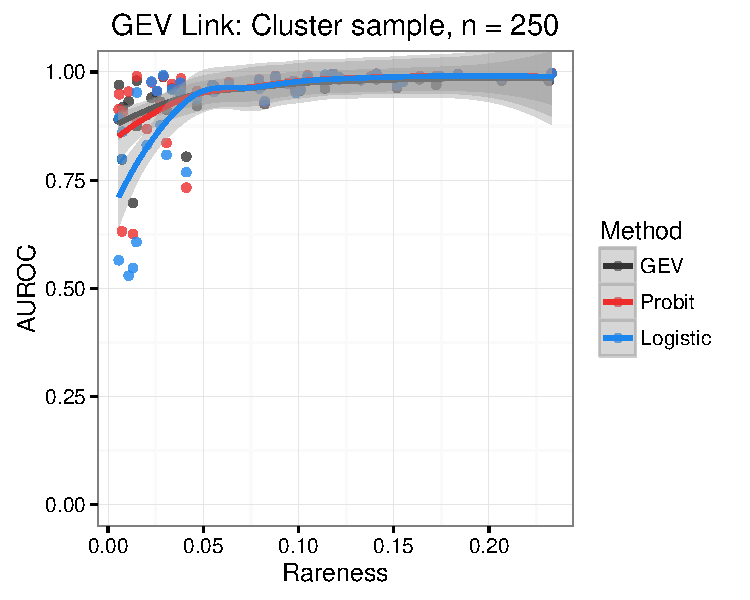
\includegraphics[width=\linewidth]{plots/byrareness-3}
  \caption{Smooth of BS (left) and AUROC (right) by rareness for GEV link and cluster sampling with $n_s = 250$.}
  \label{rbfig:simsmooth-gevclu250}
\end{figure}

\begin{figure}[htbp] % code/analysis/simstudy/combine-tables.R
  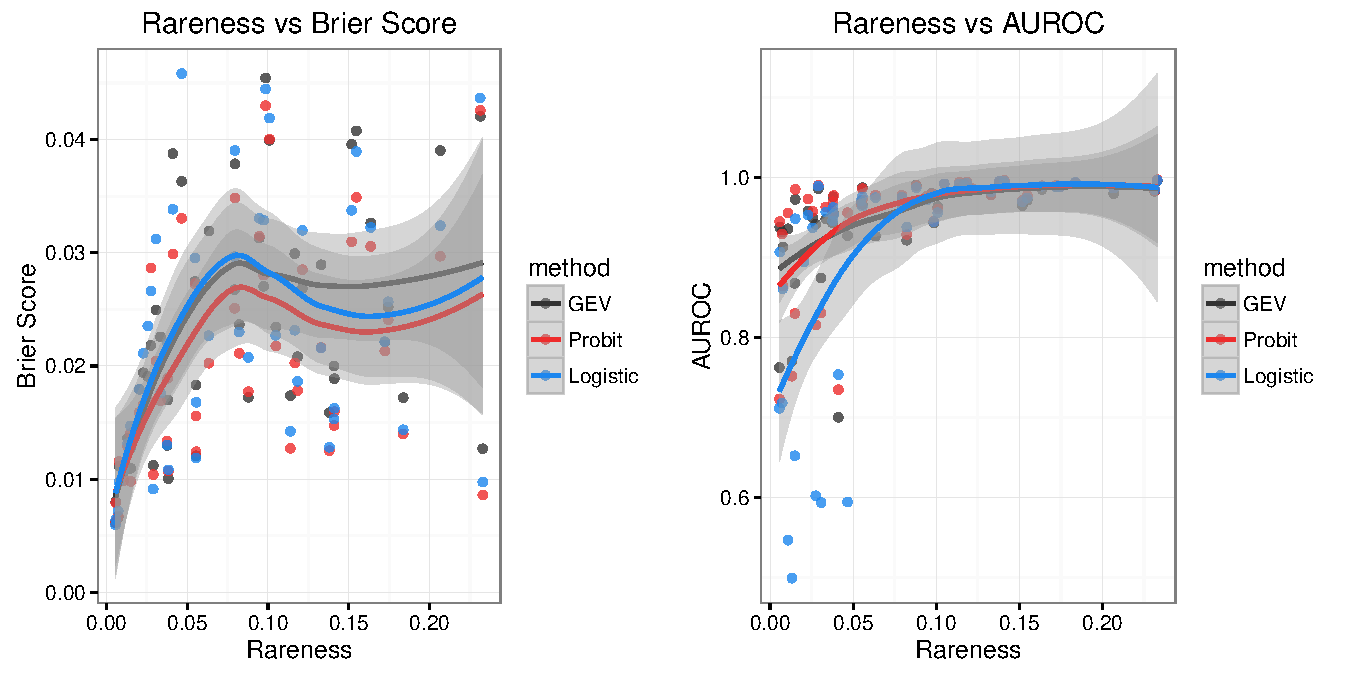
\includegraphics[width=\linewidth]{plots/byrareness-4}
  \caption{Smooth of BS (left) and AUROC (right) by rareness for GEV link and simple random sampling with $n_s = 250$.}
  \label{rbfig:simsmooth-gevsrs250}
\end{figure}

\begin{figure}[htbp] % code/analysis/simstudy/combine-tables.R
  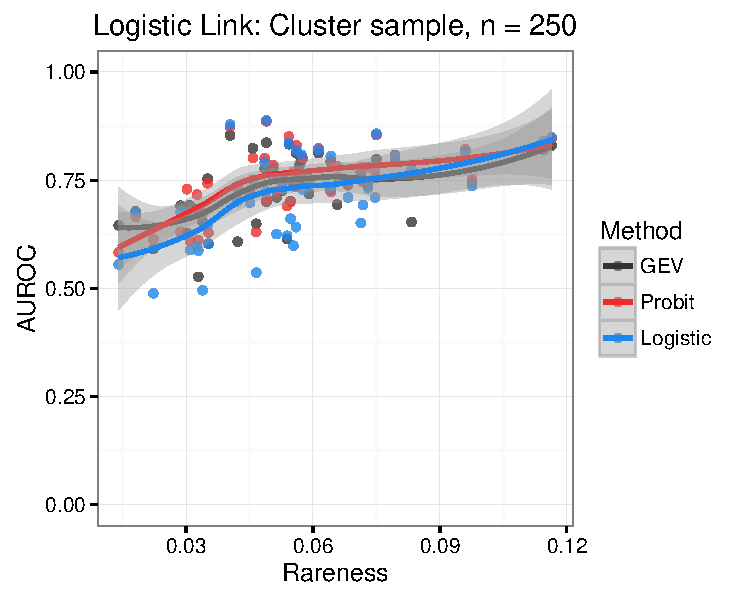
\includegraphics[width=\linewidth]{plots/byrareness-7}
  \caption{Smooth of BS (left) and AUROC (right) by rareness for logistic link and cluster sampling with $n_s = 250$.}
  \label{rbfig:simsmooth-logclu250}
\end{figure}

\begin{table}
  \caption{Brier scores ($\times 100$) [SE] and AUROC [SE] for GEV, Probit, and Logistic methods from the simulation study.}
  \label{rbtbl:simbsresults}
  \centering
  \scriptsize
  \begin{tabular}{c c c ccc c ccc}
  \toprule
    \multicolumn{3}{c}{ }& \multicolumn{3}{c}{BS} && \multicolumn{3}{c}{AUROC}\\
    \cmidrule{4-6} \cmidrule{8-10}
    Setting & $n$ & Sample & GEV & Probit & Logistic && GEV & Probit & Logistic\\
  \midrule
  GEV & 100 & CLU & 3.10 [0.27] & 2.45 [0.19] & 2.79 [0.25]
      && 0.926 [0.009] & 0.942 [0.009] & 0.900 [0.020]\\
      &     & SRS & 2.92 [0.20] & 2.54 [0.18] & 2.92 [0.25]
      && 0.938 [0.007] & 0.951 [0.007] & 0.879 [0.021]\\
      & 250 & CLU & 2.18 [0.15] & 1.87 [0.13] & 2.05 [0.14]
      && 0.951 [0.008] & 0.948 [0.011] & 0.922 [0.017]\\
      &     & SRS & 2.29 [0.15] & 2.06 [0.13] & 2.26 [0.15]
      && 0.949 [0.009] & 0.949 [0.010] & 0.908 [0.020]\\
  \midrule
  Logistic & 100 & CLU & 5.29 [0.25] & 4.94 [0.23] & 5.10 [0.25]
           && 0.659 [0.012] & 0.676 [0.014] & 0.643 [0.013]\\
           &     & SRS & 5.32 [0.23] & 5.09 [0.24] & 5.34 [0.26]
           && 0.690 [0.012] & 0.693 [0.012] & 0.613 [0.012]\\
           & 250 & CLU & 4.81 [0.21] & 4.55 [0.21] & 4.66 [0.22]
           && 0.731 [0.010] & 0.749 [0.010] & 0.714 [0.014]\\
           &     & SRS & 4.86 [0.22] & 4.63 [0.20] & 5.01 [0.23]
           && 0.742 [0.010] & 0.760 [0.010] & 0.698 [0.015]\\
  \midrule
  Hotspot & 100 & CLU & 2.29 [0.17] & 2.01 [0.15] & 1.81 [0.12]
        && 0.841 [0.016] & 0.833 [0.019] & 0.824 [0.020]\\
          &     & SRS & 2.09 [0.13] & 1.87 [0.12] & 2.13 [0.15]
          && 0.885 [0.015] &  0.906 [0.013] & 0.844 [0.015]\\
          & 250 & CLU & 1.65 [0.11] & 1.25 [0.08] & 1.40 [0.09]
          && 0.934 [0.009] &  0.949 [0.008] & 0.939 [0.011]\\
          &     & SRS & 1.53 [0.10] & 1.31 [0.08] & 1.63 [0.11]
          && 0.947 [0.007] &  0.960 [0.005] & 0.918 [0.015]\\
  \bottomrule
  \end{tabular}
\end{table}

%\begin{figure}
%  % code/analysis/simstudy/combine-tables.R
%  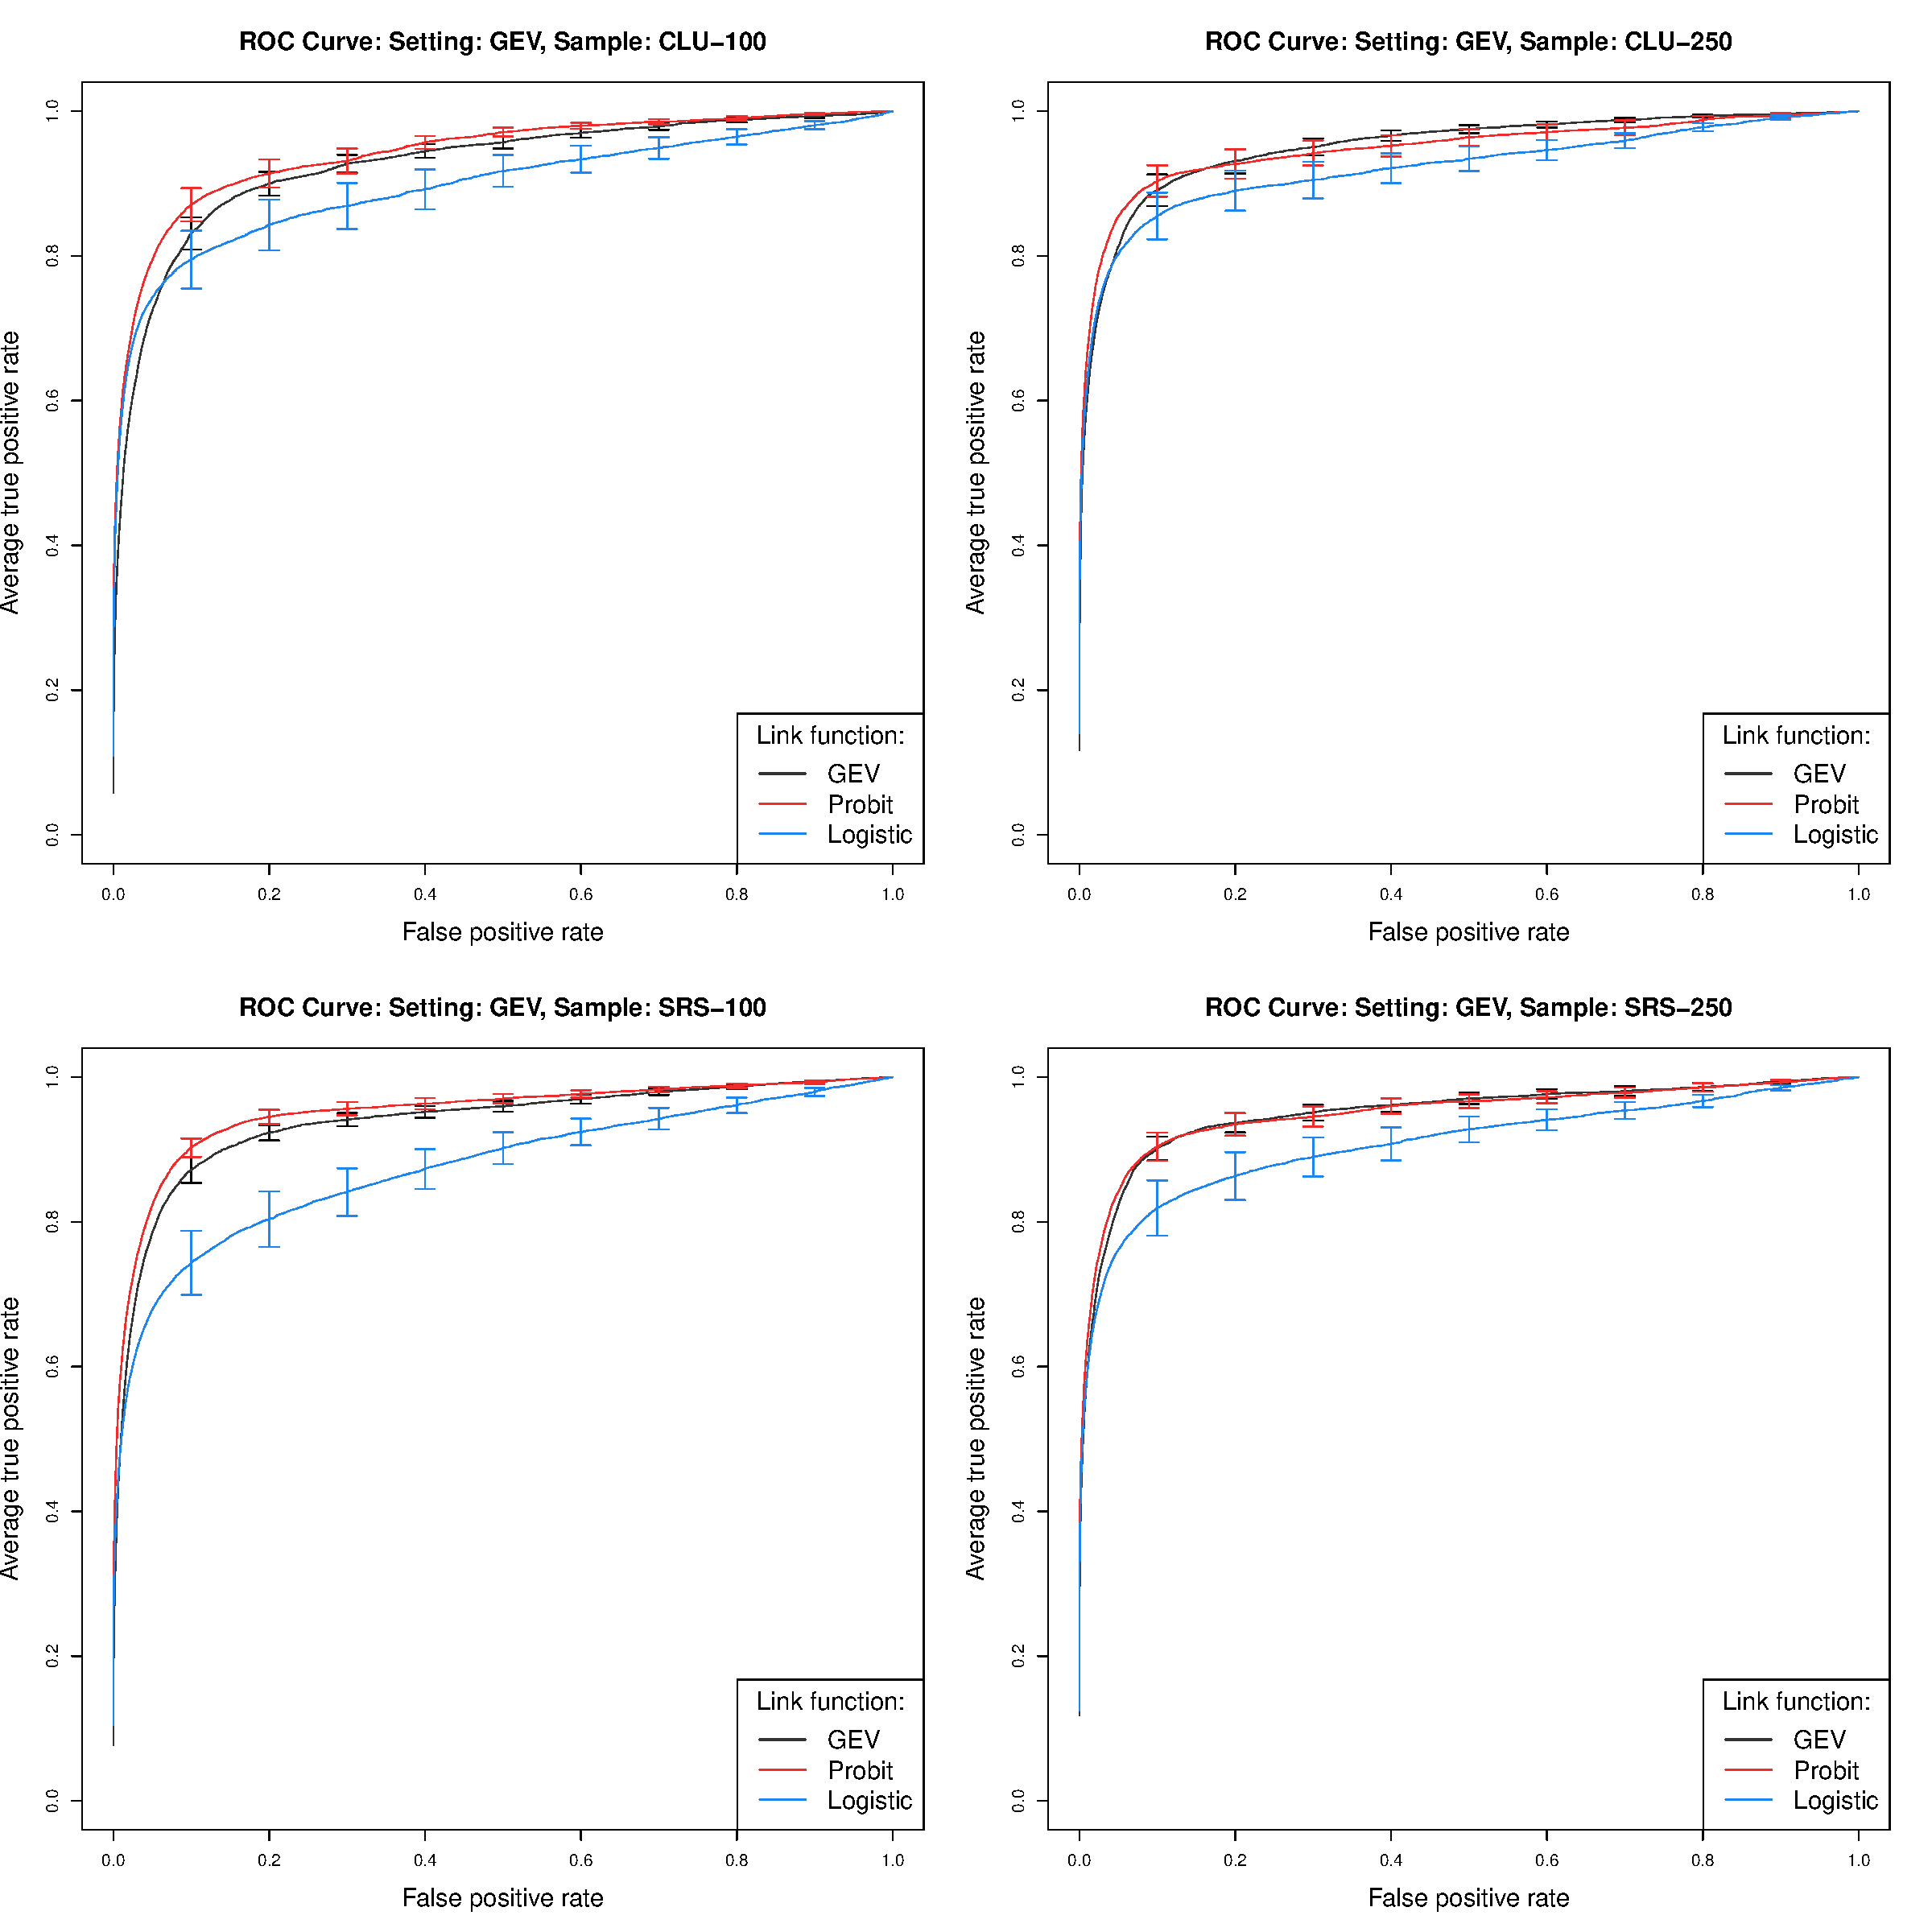
\includegraphics[width=\linewidth]{plots/sim-perf-gev}
%  \caption{Vertically averaged ROC curves for GEV simulation setting.}
%  \label{rbfig:simrocgev}
%\end{figure}
%
%\begin{figure}
%  % code/analysis/simstudy/combine-tables.R
%  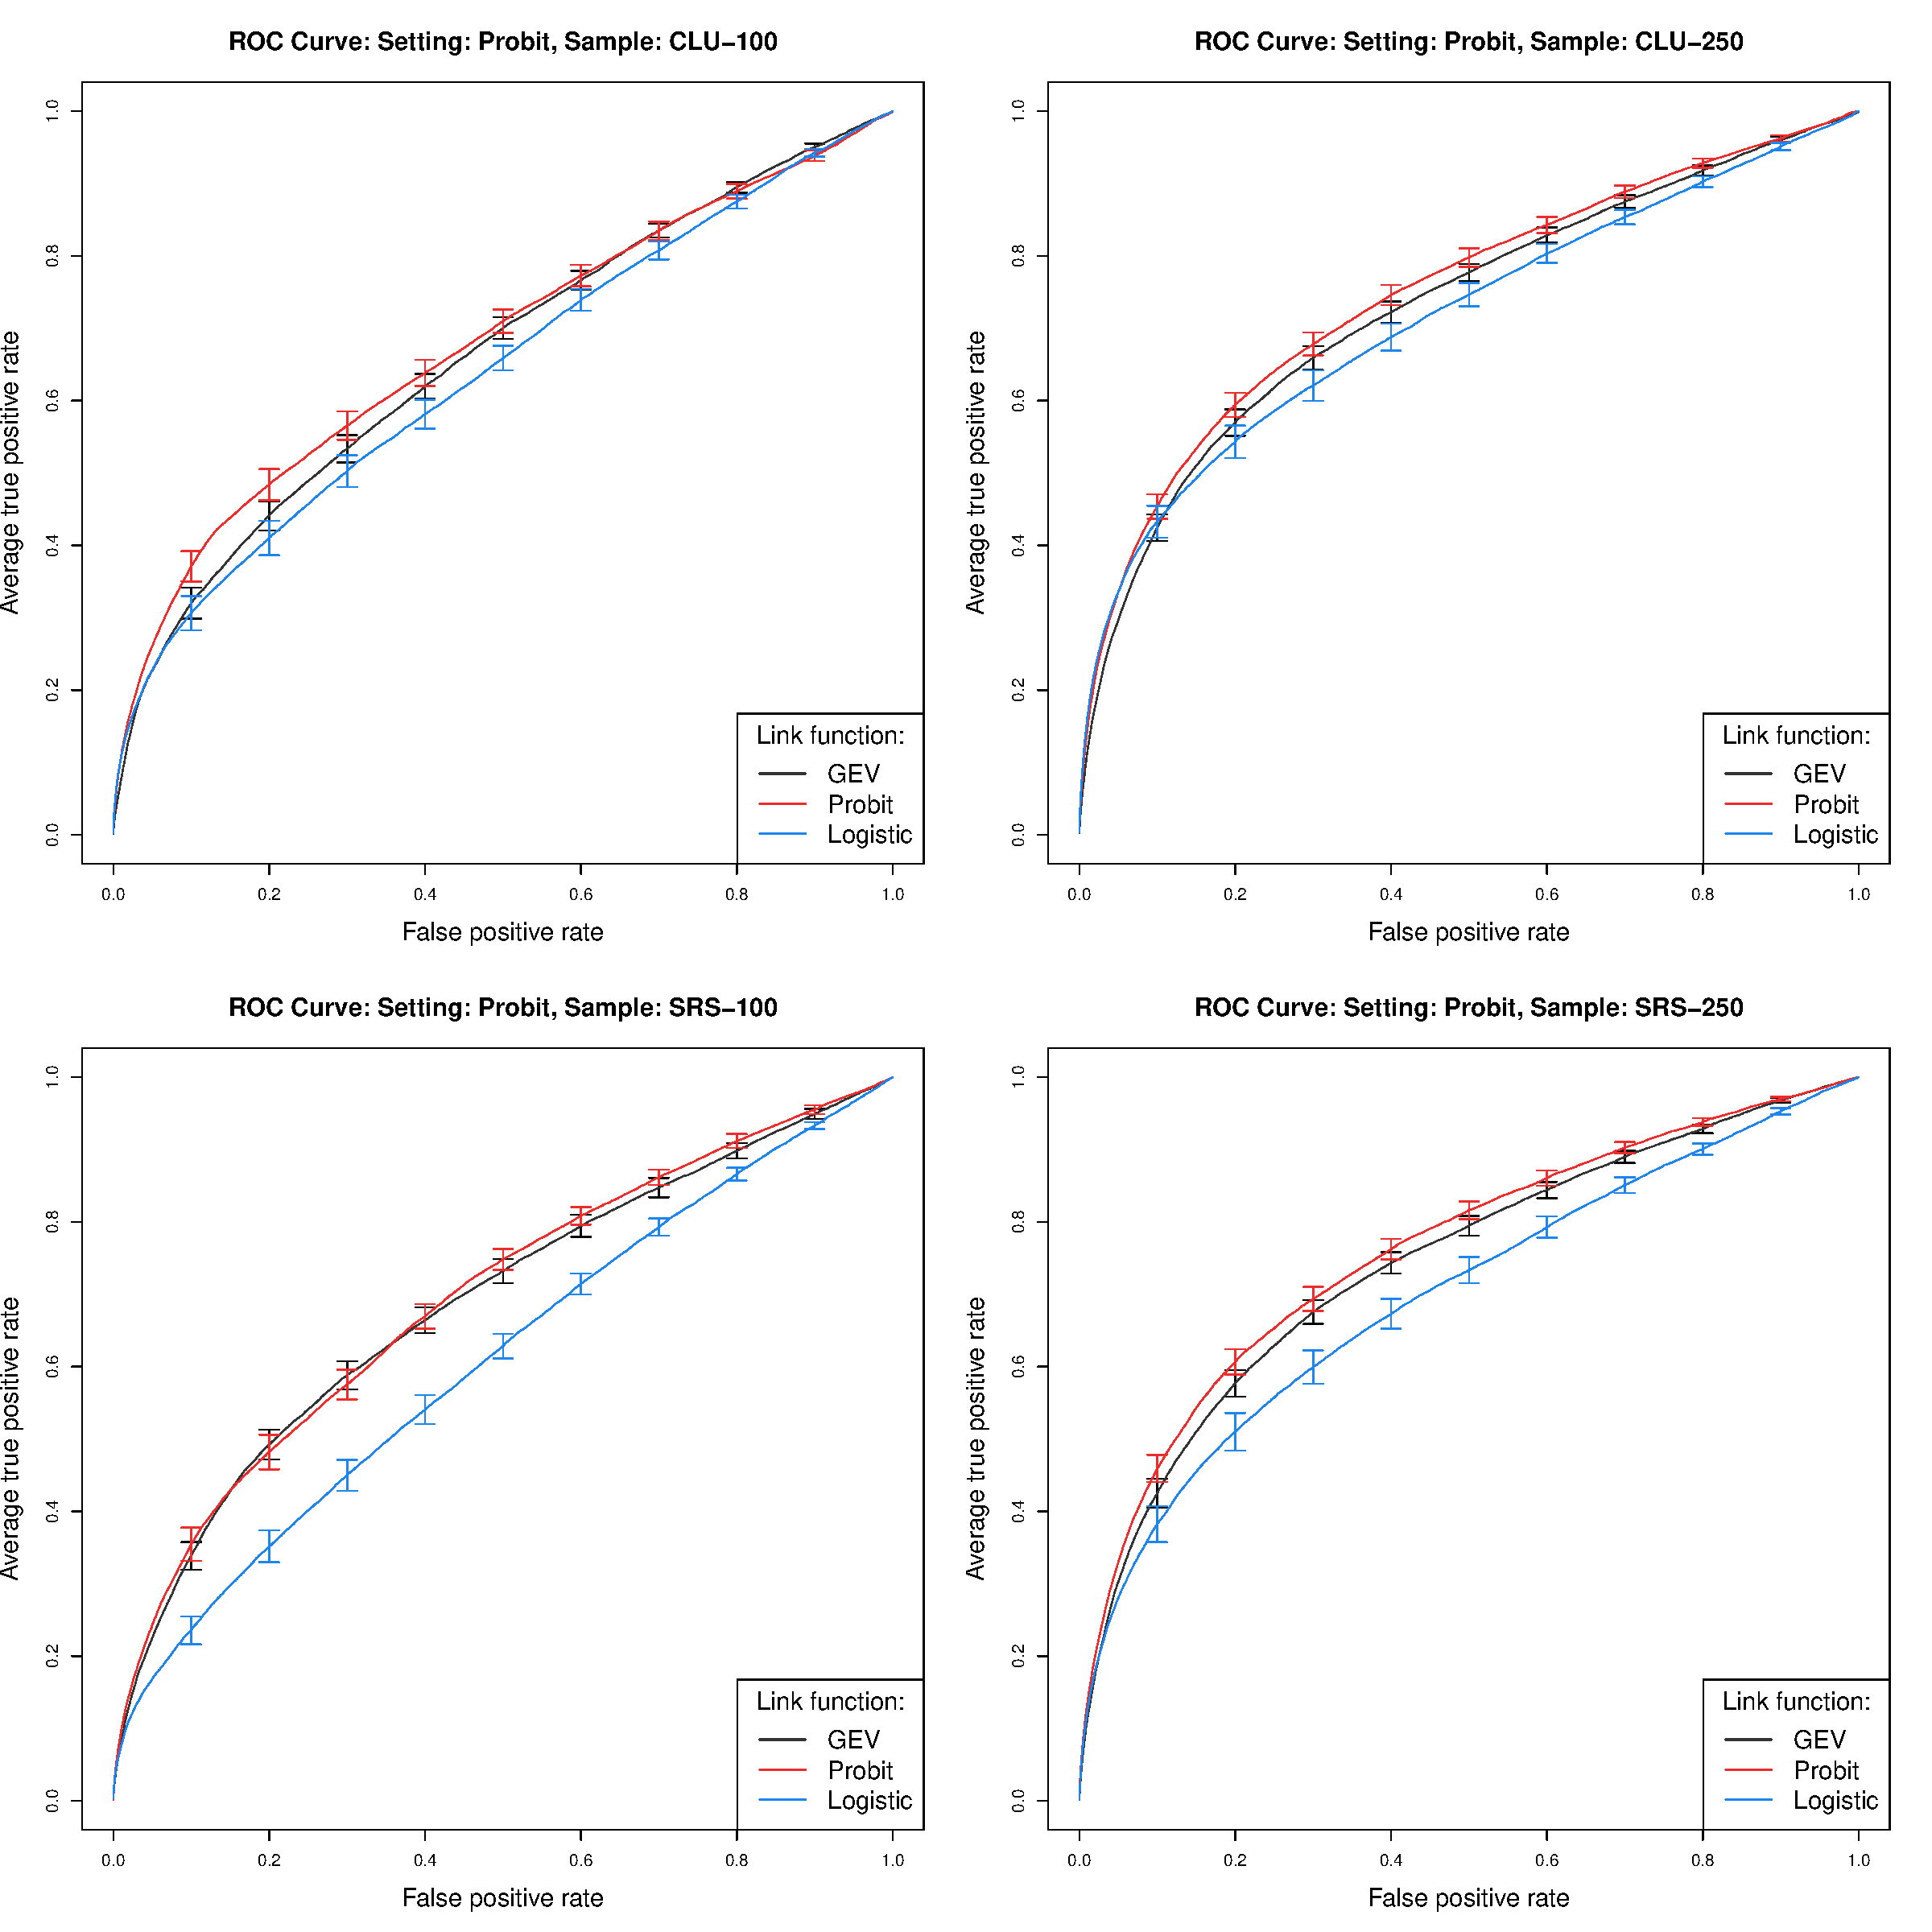
\includegraphics[width=\linewidth]{plots/sim-perf-probit}
%  \caption{Vertically averaged ROC curves for probit simulation setting.}
%  \label{rbfig:simrocpro}
%\end{figure}
%
%\begin{figure}
%  % code/analysis/simstudy/combine-tables.R
%  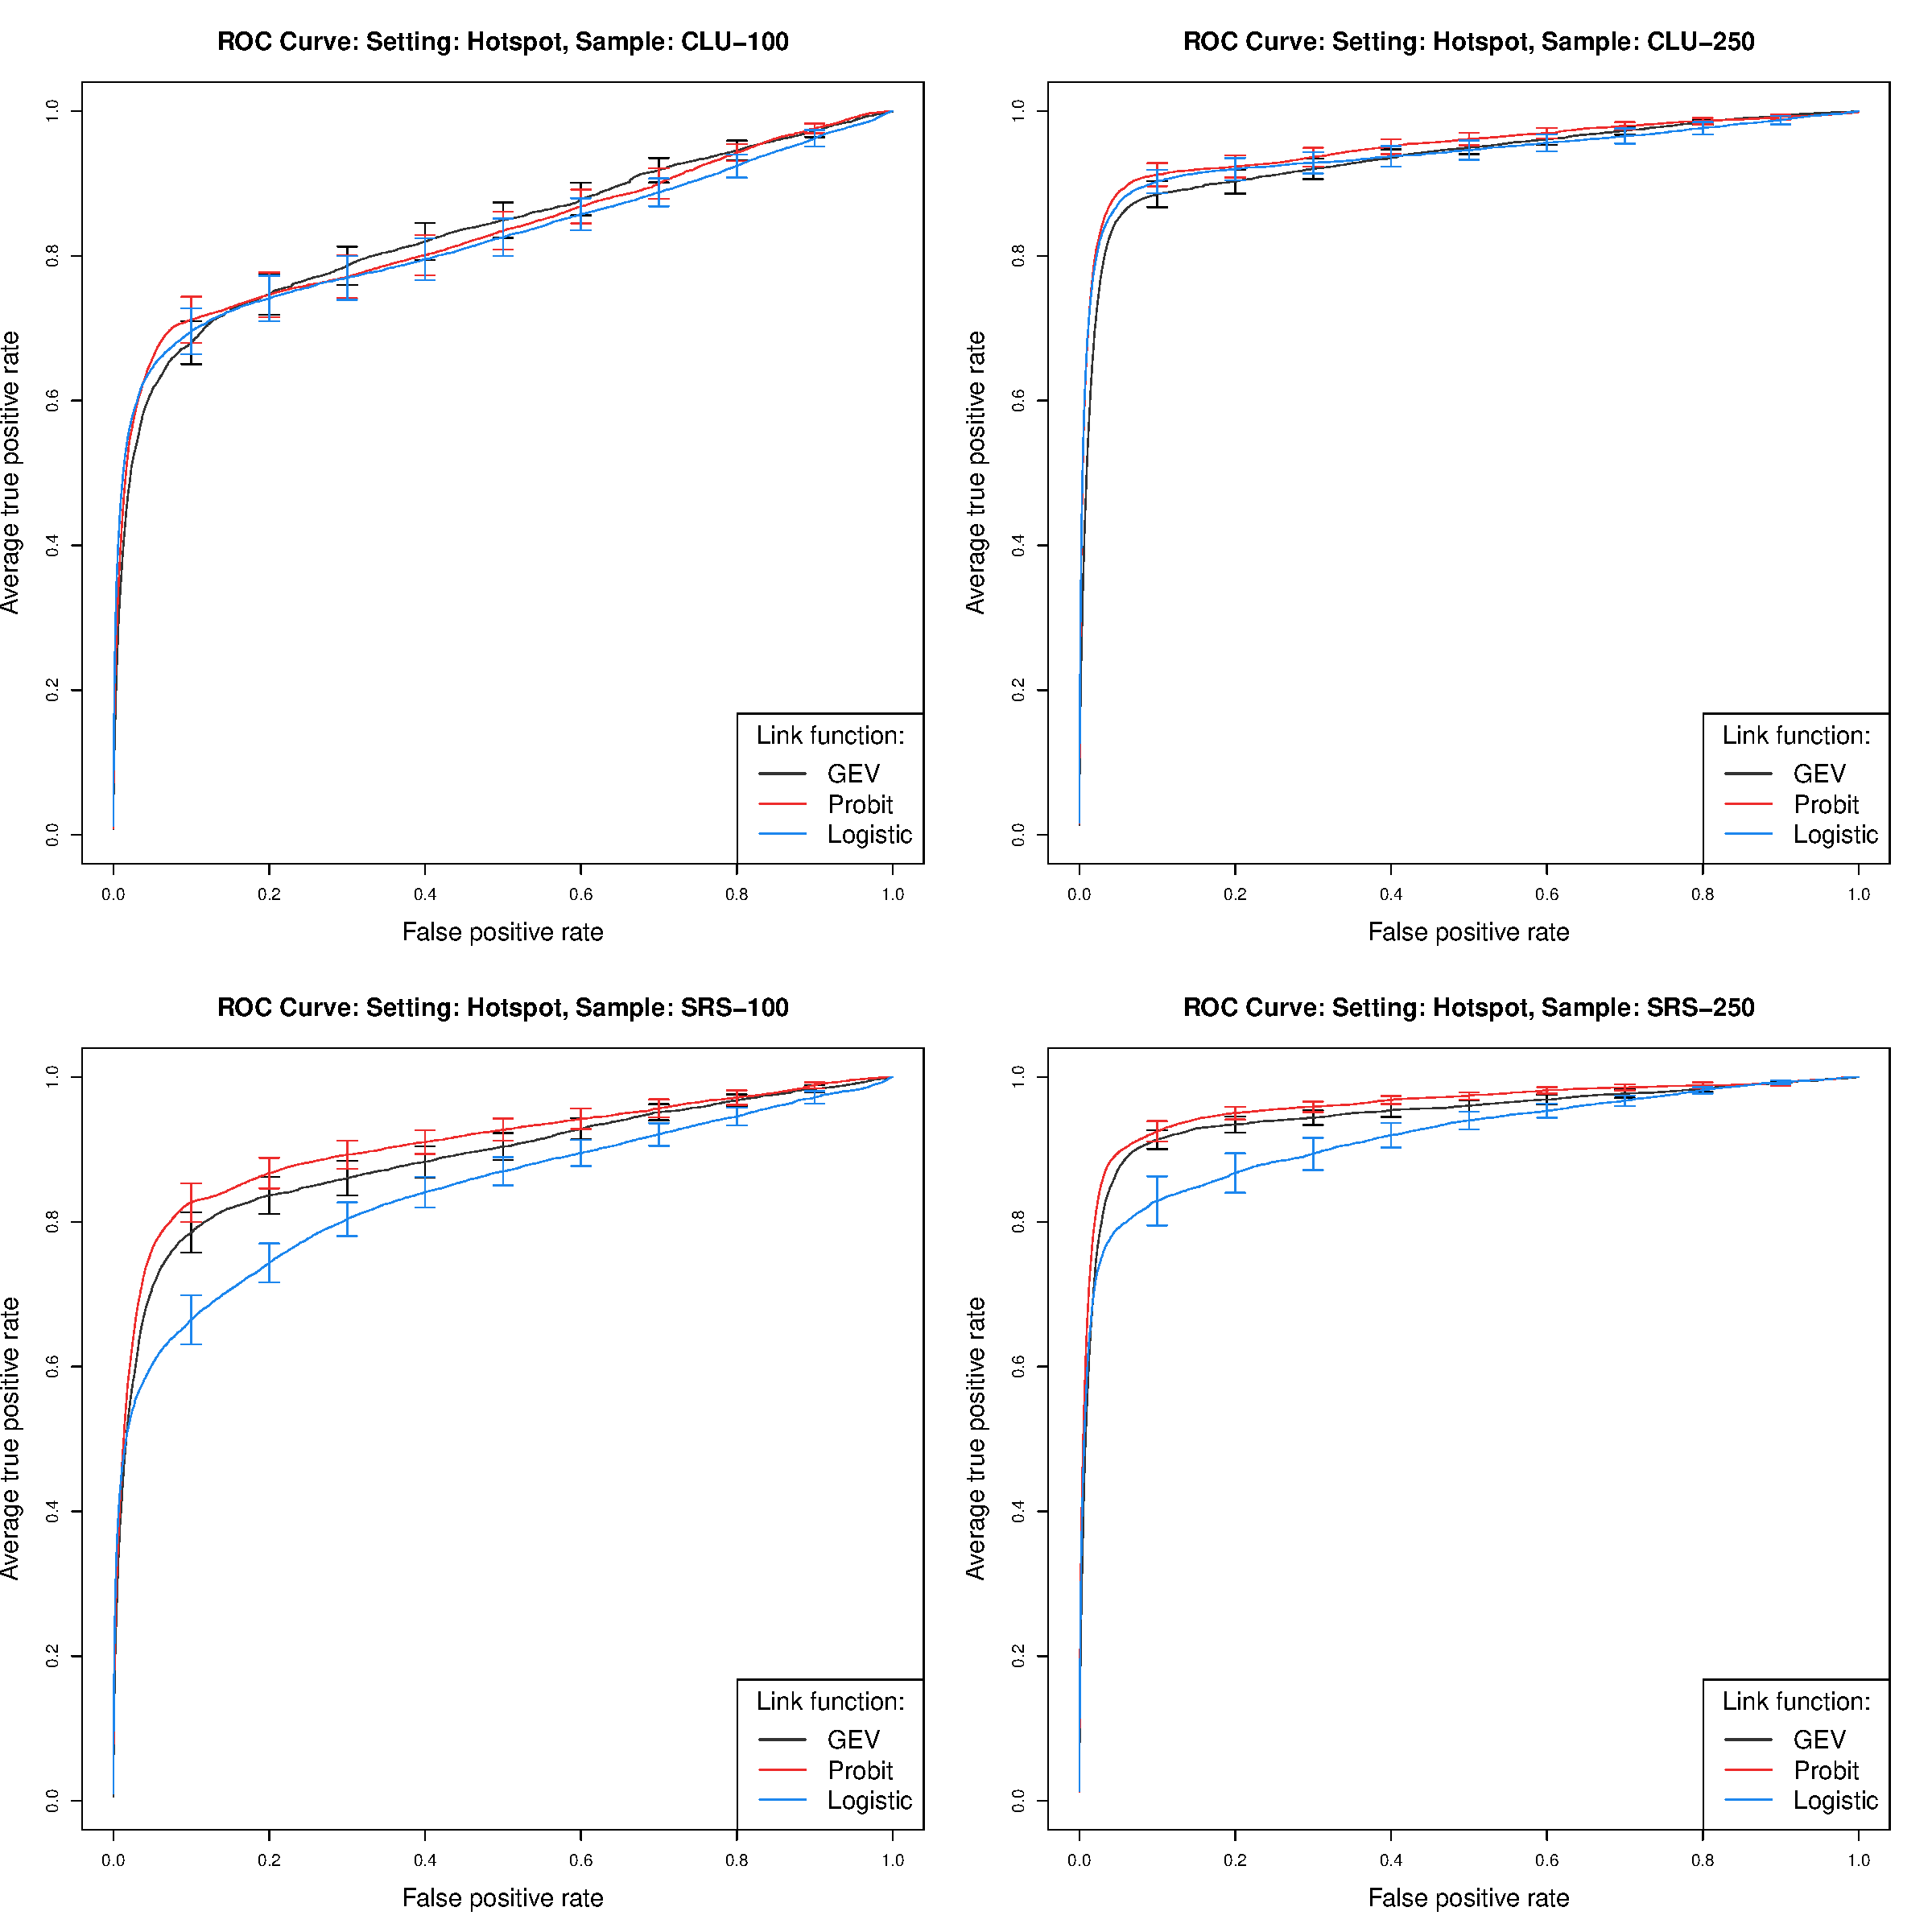
\includegraphics[width=\linewidth]{plots/sim-perf-hotspot}
%  \caption{Vertically averaged ROC curves for hotpost simulation setting.}
%  \label{rbfig:simrochot}
%\end{figure}

% \begin{table}
%   \caption{Relative AUC for GEV and Probit methods}
%   \label{rbtbl:simaucresults}
%   \centering
%   \begin{tabular}{r|lll}
%     \cline{2-4}
%               & GEV    & Probit & Logit\\
%     \hline
%     Setting 1 & 0.8998 & 0.8973 & 0.8897\\
%     Setting 2 & 0.9458 & 0.9399 & 0.9356\\
%     Setting 3 & 0.7288 & 0.7371 & 0.7157\\
%     Setting 4 & 0.7906 & 0.8056 & 0.8115\\
%     Setting 5 & 0.8426 & 0.8458 & 0.8388\\
%     Setting 6 & 0.8756 & 0.8686 & 0.8765\\
%     \hline
%   \end{tabular}
% \end{table}

% We analyzed the results for this simulation study using a Friedman test at $\alpha = 0.05$ to see if at least one method had a significantly different Brier score or AUC.
% For any setting that yielded a significant p-value, we conducted a Wilcoxon-Nemenyi-McDonald-Thompson test to see which of the methods had different results.
% The full results for the Wilcoxon-Nemenyi-McDonald-Thompson tests are given in \aref{rba:pdiffs}.
% For all settings, we find significant results for the Friedman test comparing the Brier scores for the methods.
% Specifcally, we see a statistically significant reduction in Brier score using the GEV compared to logit for settings one and two and compared to probit for setting two.
% However, in the other settings, the logit and probit methods tend to perform better than the GEV method.

% The results using AUC are much less conclusive with only settings one and four demonstrating significant differences between the methods at $\alpha = 0.05$.
% As with the Brier scores, the GEV method shows a statistically significant increase in AUC over the logit method for setting one, and for setting four, the both the probit and logit methods show a statistically significant improvement in AUC over the GEV method.

% \fref{rbfig:post-med-2} and \fref{rbfig:post-med-3} show the posterior median of $P(Y =1)$ for settings 2 and 3 respectively of a simulated dataset.
% As you can see on the figures, the both the spatial probit and logistic models oversmooth $P(Y = 1)$, whereas the spatial GEV method is able to capture small pockets of spatial dependence.
% Plots for the medians of settings 1 and 4 look similar, so they are not included here.

% \begin{figure}
%   % this figure comes from markdown/sim-hmc/predict-maps.R
%   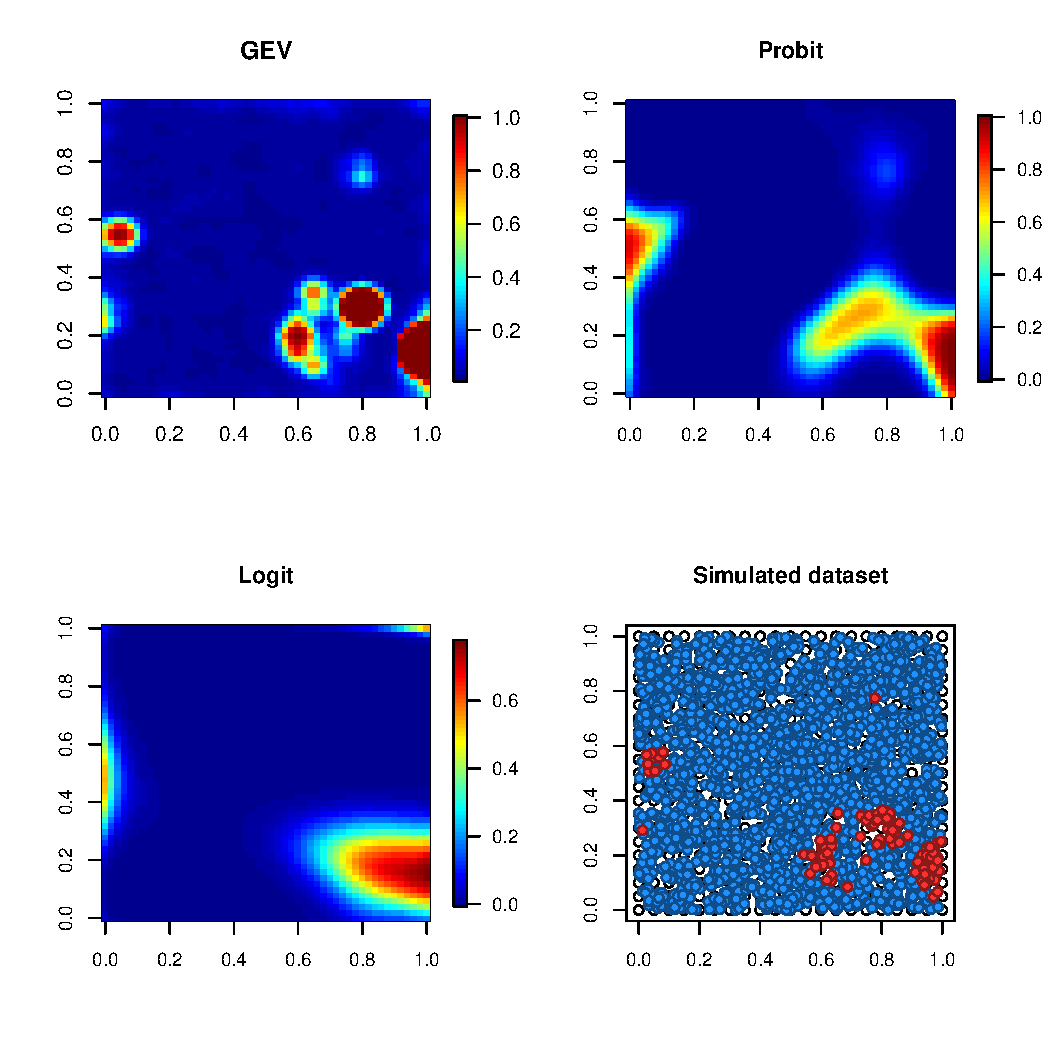
\includegraphics[width=\linewidth]{plots/post-med-2.pdf}
%   \caption{Posterior median $P(Y = 1)$ for spatial GEV, probit, and logistic regression for setting 2.}
%   \label{rbfig:post-med-2}
% \end{figure}

% \begin{figure}
%   % this figure comes from markdown/sim-hmc/predict-maps.R
%   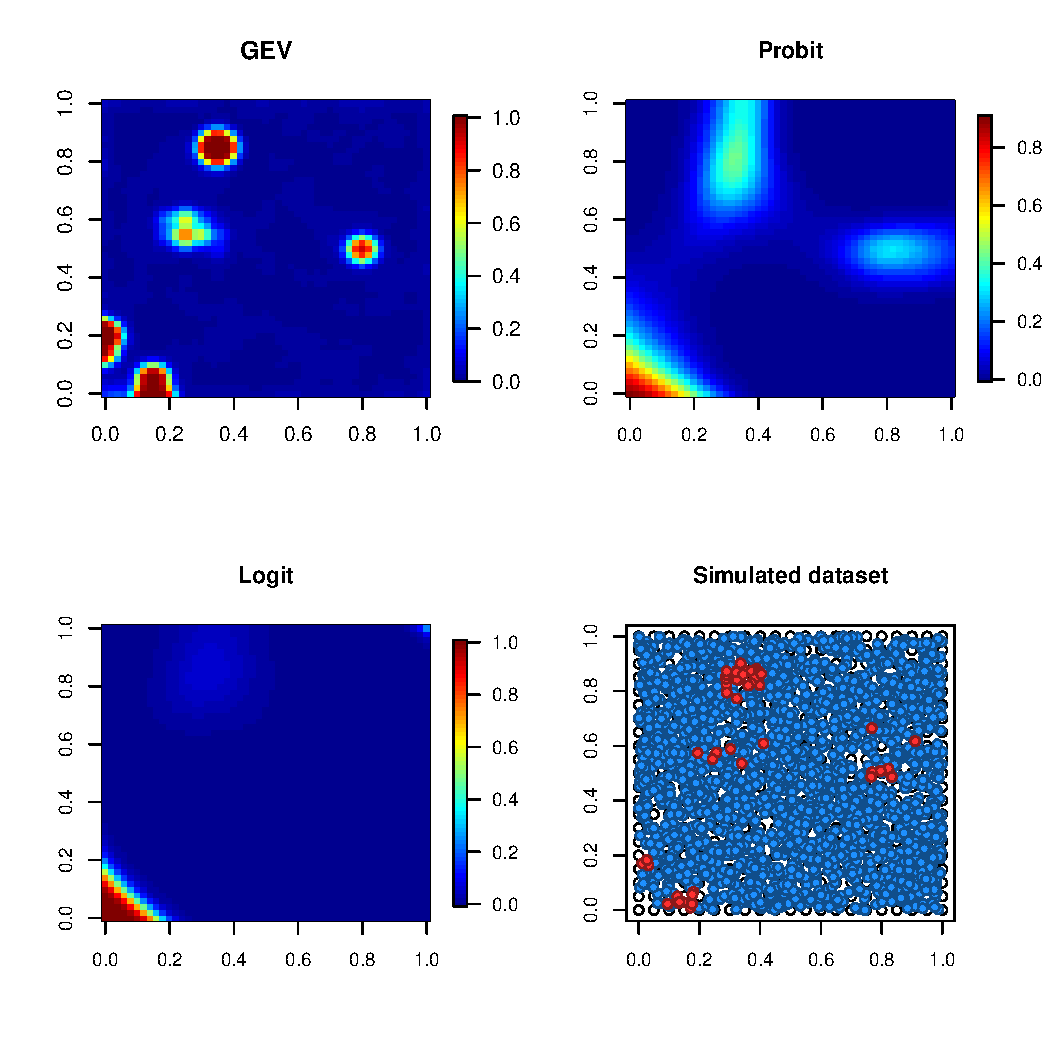
\includegraphics[width=\linewidth]{plots/post-med-3.pdf}
%   \caption{Posterior median $P(Y = 1)$ for spatial GEV, probit, and logistic regression for setting 3.}
%   \label{rbfig:post-med-3}
% \end{figure}

% If needed, species 2 is \emph{Hedysarum scoparium} , and \emph{Hedysarum scoparium} can be found in $0.54\%$ of the grid cells.

\section{Data analysis}\label{rbs:dataanalysis}

We compare our method to the spatial probit and logistic models for mapping the probability of the occurrence of \tamarix{} (TR) and \hedysarum{} (HS), two  plant species, for a 1-km$^2$ study region of PR China \citep{Smith2012}.
The Chinese Academy of Forestry conducted a full census of the area, and the true occupancy of the species are plotted in \fref{rbfig:occupancy}.
\begin{figure}
  \centering
  \includegraphics[width=\linewidth, trim=0 10em 0 10em]{plots/plant-census.pdf}
  \caption{True occupancy of \tamarix (left) and \hedysarum (right) from a 1-km$^2$ study region of PR China.}
  \label{rbfig:occupancy}
\end{figure}
The region is split into $10$-m $\times$ $10$-m grid cells.
\tamarix{} can be found in approximately $6\%$ of the grid cells, and \hedysarum{} can be found in approximately $0.54\%$ of the grid cells.

\subsection{Methods} \label{rbs:datamethods}

For the data analysis, we generate 50 subsamples using the CLU and SRS sampling methods with $n_s = 100$, $250$ initial locations.
For each subsample, we fit the spatial GEV, spatial probit, and spatial logistic models.
Knot placement, prior distributions, and MCMC details for the data analysis are the same as the simulation study.
To compare models, we use similar metrics as in the simulation study, but we average the metrics over subsamples.

\subsection{Results}\label{rbs:dataresults}

As with the simulation study, we find that in most cases the spatial probit model gives the best performance.
\tref{rbtbl:dataresults} give summary Brier scores ($\times 100$) and AUROC for the \tamarix{} and \hedysarum{} analysis along with the time (in seconds) for 1,000 iterations of the MCMC sampler.
These timings come from a single core of an Intel Core i7-5820K Haswell-E processor, using the OpenBLAS optimized BLAS library (\url{http://www.openblas.net}).
\fref{rbfig:data1roc} gives the vertically averaged ROC curves for each method and sampling setting for \tamarix{} and \fref{rbfig:data2roc} gives the vertically averaged ROC curves for \hedysarum{}.
These results appear to support the suggestion from the simulation study that spatial GEV gives an advantage as rareness increases.
For \tamarix, when $n = 100$, there is a small distinction between the spatial GEV and probit models.
The results suggest that the GEV model has a small improvement over probit in the case of cluster sampling, but that using a probit model demonstrates a small improvement over the GEV model in the simple random setting.
However, when $n = 250$, both logistic and probit models appear to outperform the GEV model.
For the rarer species, \hedysarum, we find more conclusive evidence that the GEV model provides an improvement for cluster sampling when $n = 100$.
At this sample size, there is also some evidence to suggest that the GEV model gives some improvement over the probit model for simple random sampling.
For $n = 250$, we still have evidence that using a cluster sampling strategy, the GEV model gives the best performance, but for simple random sampling, the probit model performs the best.

\section{Discussion and future research}\label{rbs:conclusions}

In this paper, we present a max-stable spatial method for rare binary data.
The principal finding in this paper is that the spatial probit model tends to outperform the proposed model.
This finding is surprising given that the max-stable process is the theoretically justified spatial process for extreme value distributions, and it leads to possible research questions in the future.

It is unusual that the spatial probit model should outperform the proposed model, particularly when the data are generated directly from the proposed model.
One possible explanation is that for the simulated data, there is a wide range of rarity in the data (GEV: $0.5\%$ -- $35.9\%$, Logistic: $1.4\%$ -- $14.4\%$, and Hotspot: $0.5\%$ -- $6.8\%$).
Given that for both the GEV and logistic data settings, we have a number of datasets with a relatively high rate of occurrence, it is possible that probit is competitive partly due to the fact that the data are not rare.
Both the simulation study and data analysis appear to support the idea that the GEV method will perform better on rarer datasets.
Therefore, it may be useful to conduct more research on rare datasets or through simulation with a slightly more restrictive data generation strategy (i.e. restrict datasets to $K < 500$).

\begin{figure}
  % code/analysis/swd/combine-tables.R
  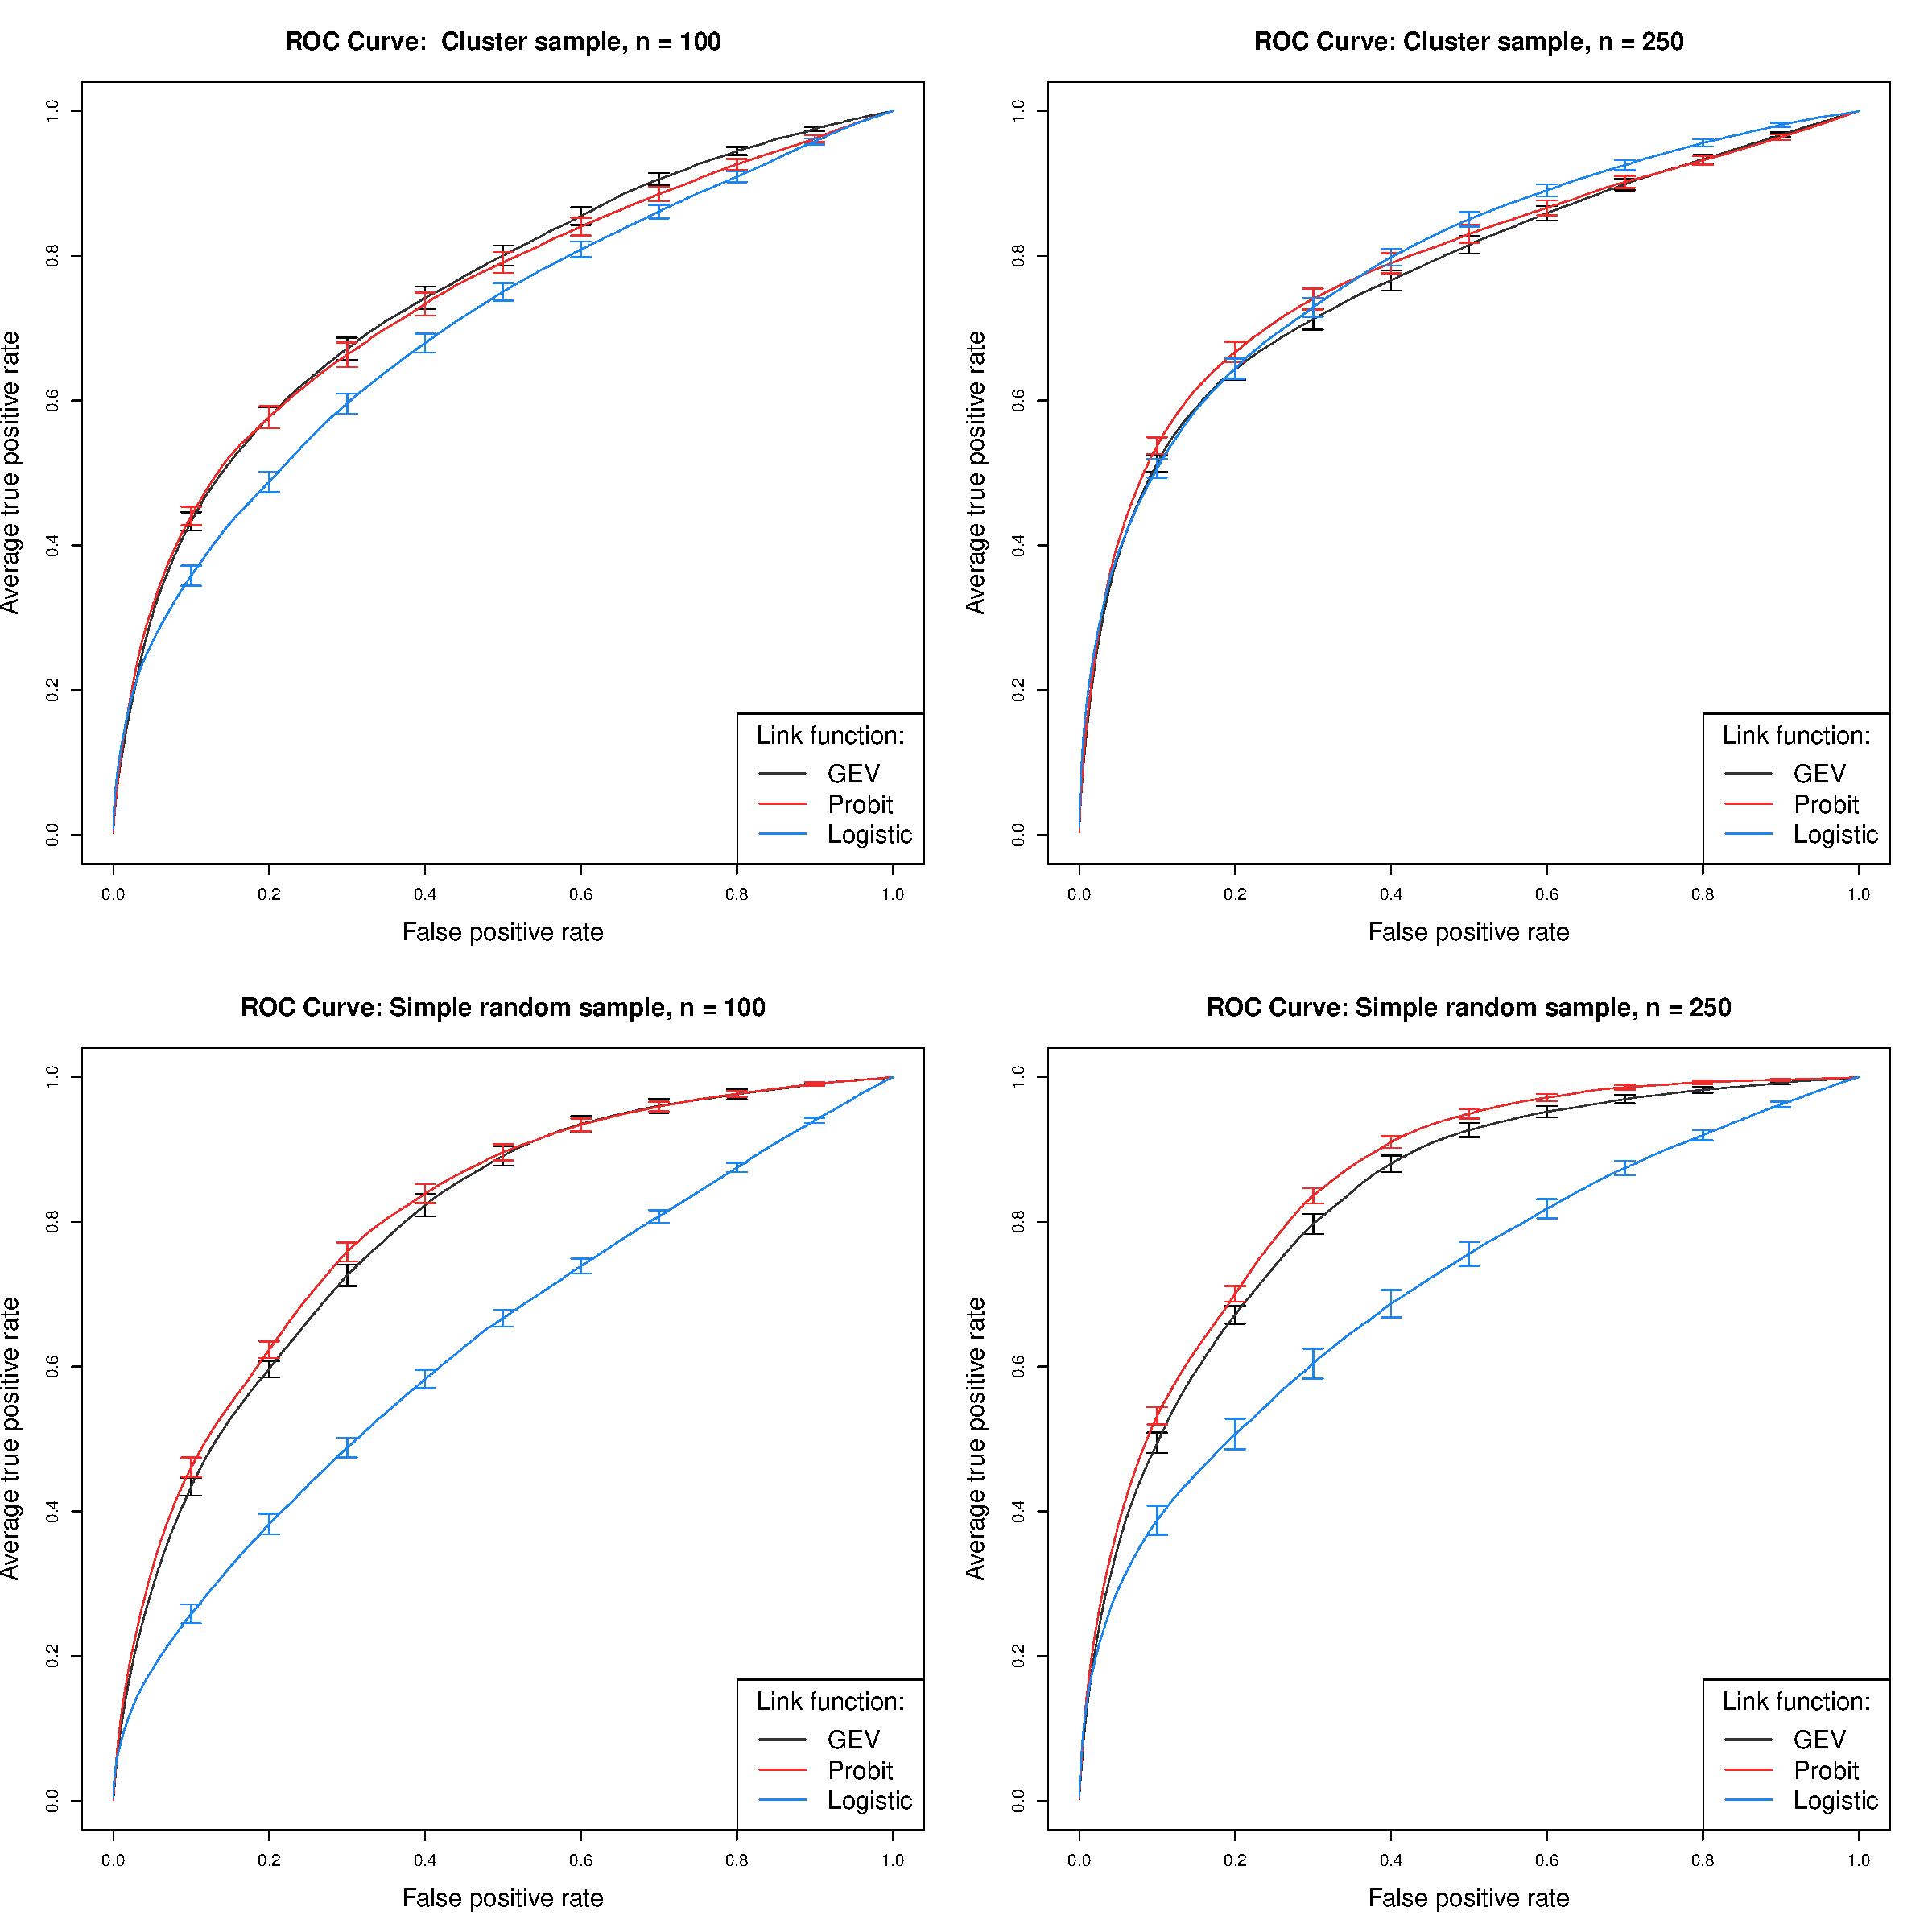
\includegraphics[width=\linewidth]{plots/data-perf-species1}
  \caption{Vertically averaged ROC curves for \emph{Tamarix ramosissima}.}
  \label{rbfig:data1roc}
\end{figure}

\begin{figure}
  % code/analysis/swd/combine-tables.R
  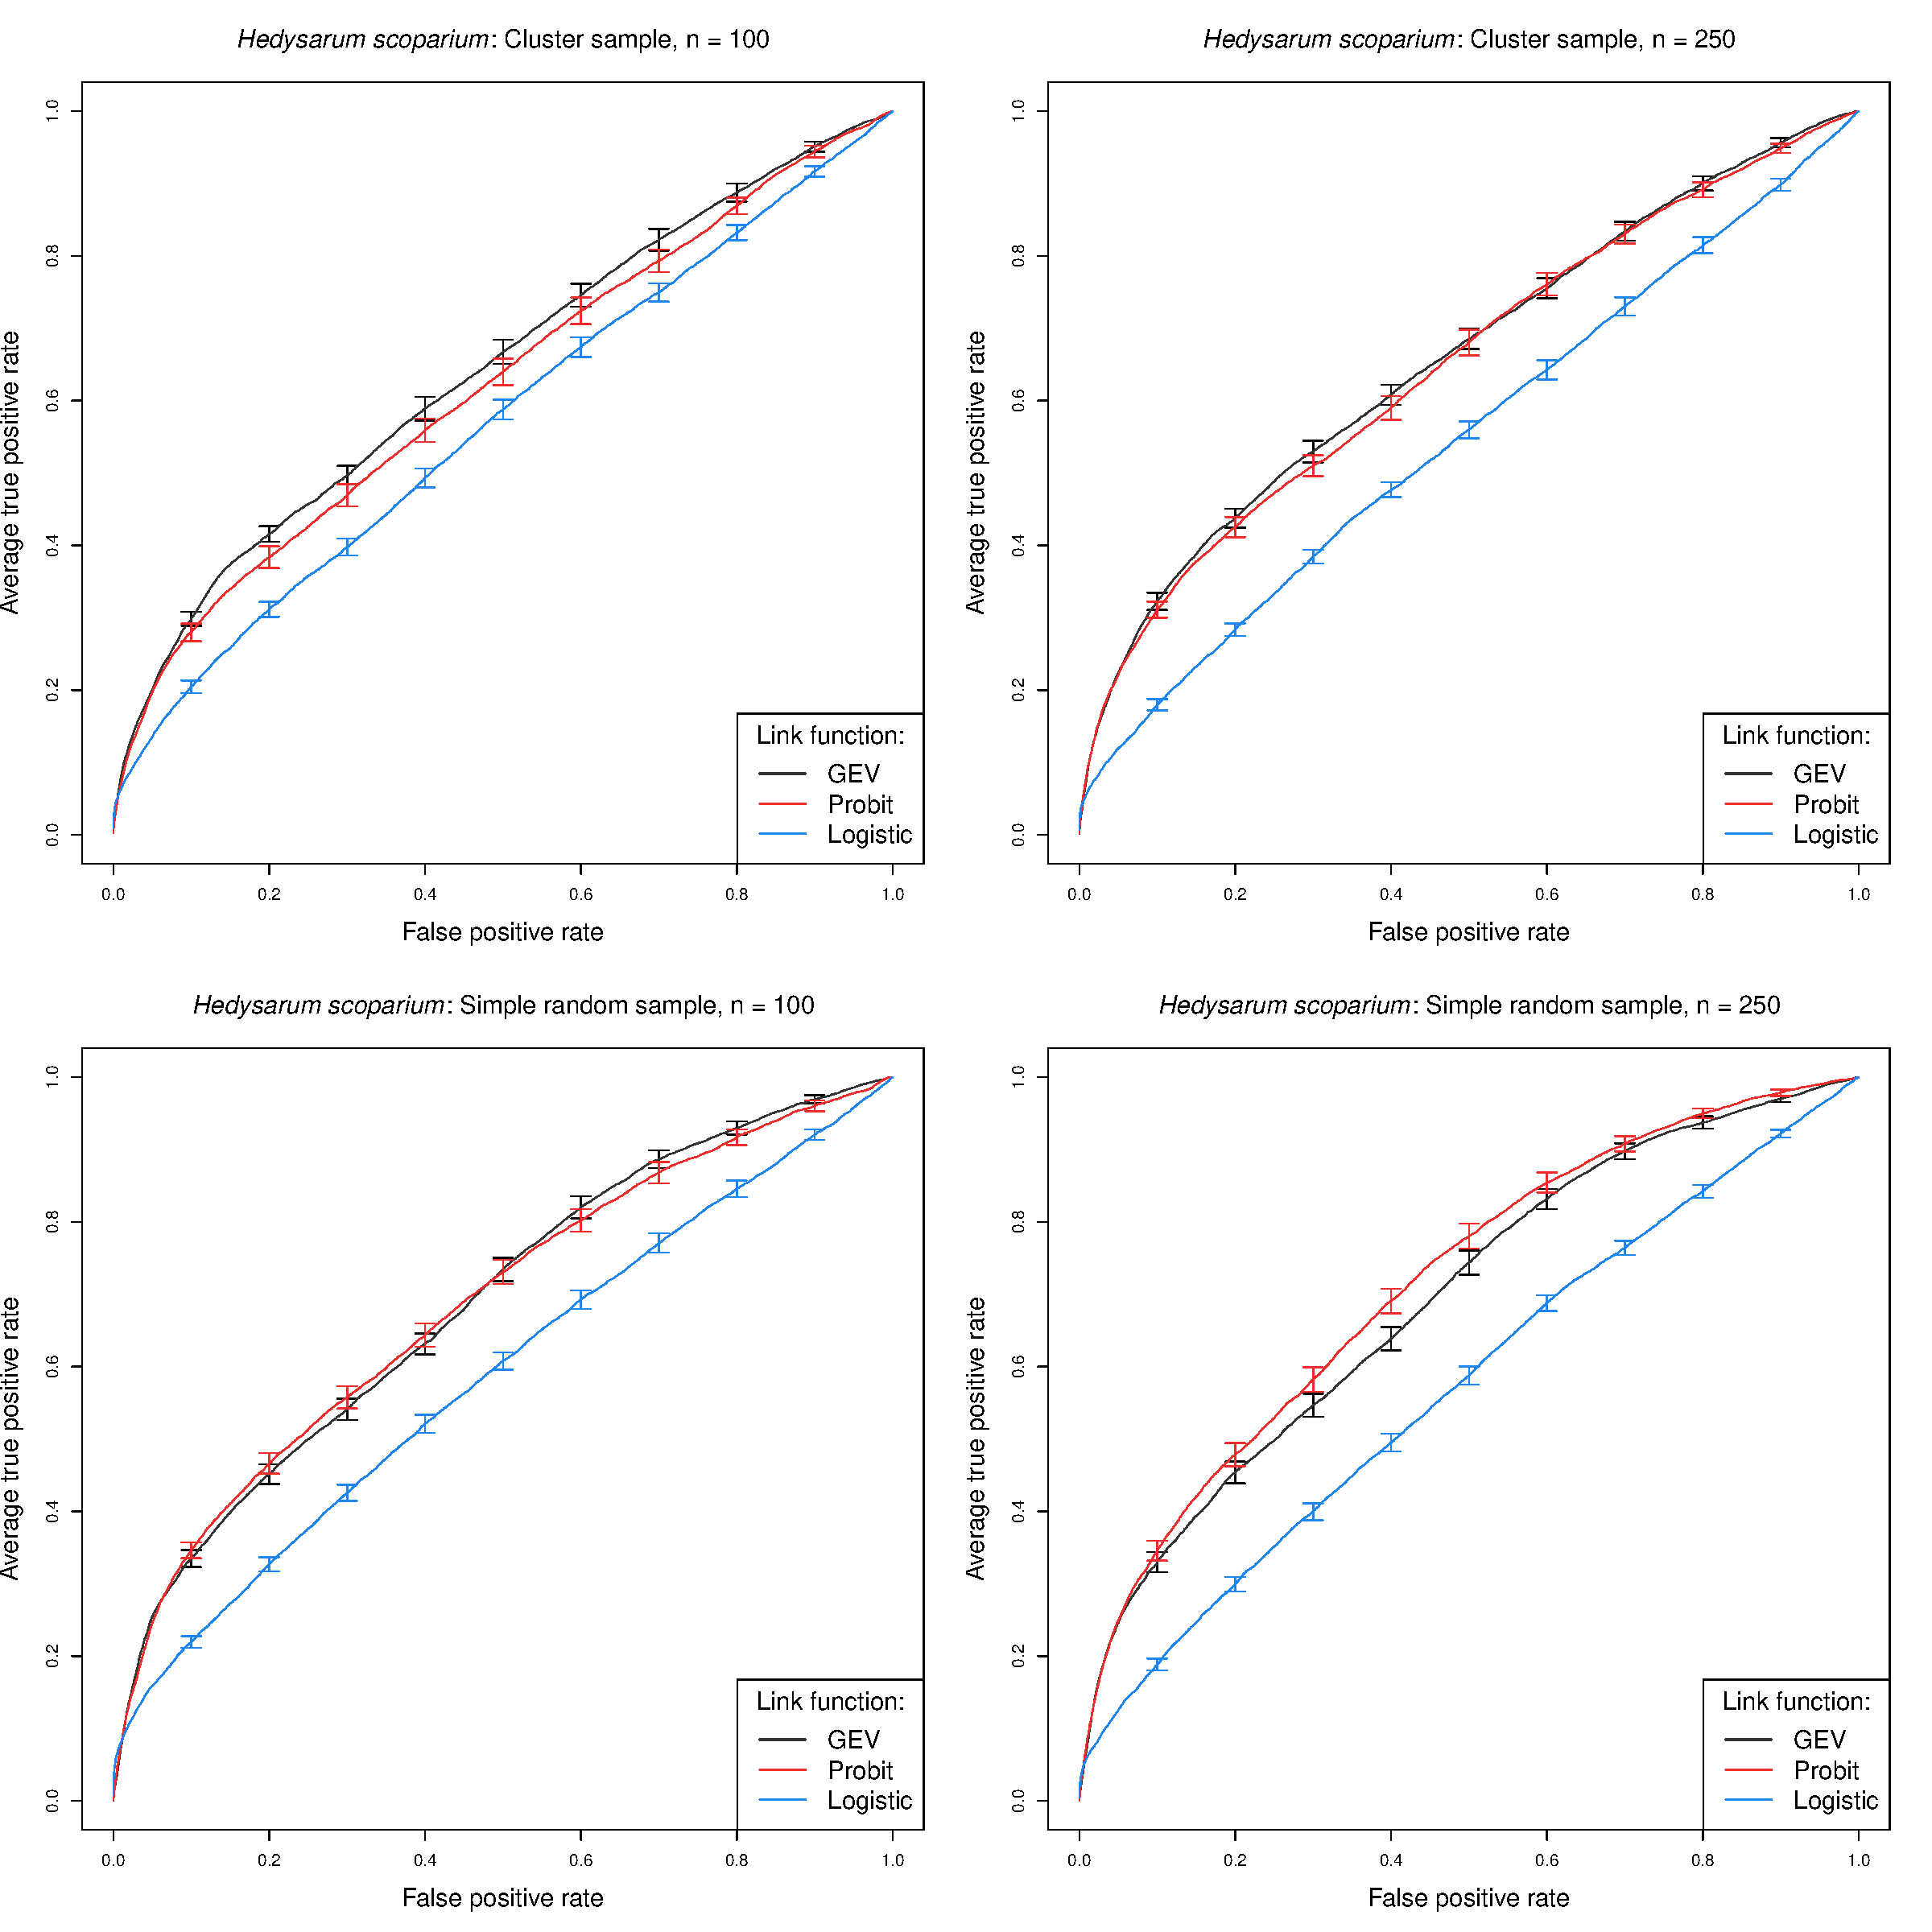
\includegraphics[width=\linewidth]{plots/data-perf-species2}
  \caption{Vertically averaged ROC curves for \emph{Hedysarum scoparium}.}
  \label{rbfig:data2roc}
\end{figure}

\begin{landscape}
\begin{table}
  \caption{Brier scores ($\times 100$) [SE], AUROC [SE], and time (in seconds) for 1,000 iterations of GEV, Probit, and Logistic methods for \tamarix{} and \hedysarum{}.}
  \label{rbtbl:dataresults}
  \centering
  \scriptsize
  \subfloat[\tamarix{}]{
    \begin{tabular}{c c ccc c ccc c rrr}
    \toprule
      \multicolumn{2}{c}{ }& \multicolumn{3}{c}{BS} && \multicolumn{3}{c}{AUROC} && \multicolumn{3}{c}{Time} \\
      \cmidrule{3-5} \cmidrule{7-9} \cmidrule{11-13}
      $n$ & Samp. & GEV    & Probit & Logistic && GEV    & Probit & Logistic && GEV    & Probit & Logistic \\
    \midrule
    100 & CLU & 5.120 [0.050] & 5.039 [0.049] & 5.382 [0.029]
        && 0.732 [0.014] & 0.731 [0.014] & 0.699 [0.012]
        && 6.1 & 1.1 & 2.4\\
        & SRS & 4.997 [0.045] & 4.938 [0.055] & 5.500 [0.027]
        && 0.798 [0.008] & 0.802 [0.009] & 0.636 [0.012]
        && 6.2 & 1.1 & 2.6\\
    250 & CLU & 4.779 [0.049] & 4.657 [0.045] & 4.950 [0.051]
        && 0.771 [0.013] & 0.784 [0.013] & 0.798 [0.011]
        &&  &  & \\
        & SRS & 4.823 [0.053] & 4.735 [0.048] & 5.120 [0.071]
        && 0.827 [0.011] & 0.851 [0.007] & 0.717 [0.019]
        &&  &  & \\
    \bottomrule
    \end{tabular}
  }

  \subfloat[\hedysarum]{
    \begin{tabular}{c c ccc c ccc c rrr}
      \toprule
      \multicolumn{2}{c}{ }& \multicolumn{3}{c}{BS} && \multicolumn{3}{c}{AUROC} && \multicolumn{3}{c}{Time}\\
      \cmidrule{3-5} \cmidrule{7-9} \cmidrule{11-13}
      $n$ & Samp. & GEV    & Probit & Logistic && GEV    & Probit & Logistic && GEV    & Probit & Logistic \\
      \midrule
      100 & CLU & 1.765 [0.018] & 1.831 [0.029] & 1.679 [0.002]
          && 0.642 [0.010] & 0.617 [0.012] & 0.573 [0.008]
          && 5.7 & 1.0 & 2.1\\
          & SRS & 1.914 [0.066] & 1.996 [0.083] & 1.685 [0.002] && 0.686 [0.009] & 0.683 [0.011] & 0.587 [0.008]
          && 5.7 & 1.0 & 2.2\\
      250 & CLU & 1.667 [0.005] & 1.657 [0.006] & 1.679 [0.001]
          && 0.659 [0.009] & 0.648 [0.011] & 0.566 [0.005]
          &&  &  & \\
          & SRS & 1.691 [0.017] & 1.666 [0.010] & 1.684 [0.001] && 0.691 [0.010] & 0.709 [0.012] & 0.574 [0.007]
          &&  &  & \\
      \bottomrule
    \end{tabular}
  }
\end{table}
\end{landscape}

\section*{Acknowledgments}

\appendix
\section{Appendices}
\subsection{Binary regression using the GEV link} \label{rba:rarebinary}
Here, we provide a brief review of the the GEV link of \citet{Wang2010}.
Let $Y_i \in \{0, 1\}, i = 1, \ldots, n$ be a collection of i.i.d. binary responses.
It is assumed that $Y_i = I(z_i > 0)$ where $I(\cdot)$ is an indicator function, $z_i = [1 - \xi \bX_i \bbeta]^{1 / \xi}$ is a latent variable following a GEV$(1, 1, 1)$ distribution, $\bX_i$ is the associated $p$-vector of covariates with first element equal to one for the intercept, and $\bbeta$ is a $p$-vector of regression coefficients.
Then, $Y_i \ind$ Bern$(\pi_i)$ where $\pi_i= 1 - \exp \left( -\frac{ 1 }{ z_i } \right)$.


\subsection{Derivation of the likelihood} \label{rba:likelihoodderivation}
We use the hierarchical max-stable spatial model given by \citet{Reich2012}. If at each margin, $Z_i \sim $ GEV$(1,1,1)$, then $Z_i | \theta_i \indep $ GEV$(\theta, \alpha \theta, \alpha)$. We reorder the data such that $Y_1=\ldots=Y_K=1$, and $Y_{K+1} = \ldots = Y_n = 0$. Then the joint likelihood conditional on the random effect $\theta$ is

\begin{align} \label{rbeq:joint_cond}
	P(Y_1=y_1,\ldots,Y_n=y_n) =& \prod_{ i \le K } \left\{ 1 - \exp \left[ - \left( \frac{ \theta_i }{ z_i } \right)^{ 1/\alpha} \right] \right \} \prod_{ i > K } \exp \left[ -\left( \frac{ \theta_i }{ z_i } \right)^{1/\alpha} \right] \nonumber \\[0.5em]
		=& \exp \left[ -\sum_{ i = K+1}^{ n }\left( \frac{ \theta_i }{ z_i } \right)^{1/\alpha} \right] - \exp \left[ -\sum_{ i = K+1}^{ n }\left( \frac{ \theta_i }{ z_i } \right)^{1/\alpha} \right] \sum_{ i = 1}^{K} \exp\left[ -\left( \frac{ \theta_i }{ z_i } \right)^{ 1/\alpha} \right] \nonumber\\
		&  + \exp \left[ -\sum_{ i = K+1}^{ n }\left( \frac{ \theta_i }{ z_i } \right)^{1/\alpha} \right] \sum_{ 1 < i < j \le K } \left\{ \exp \left[ - \left( \frac{ \theta_i }{ z_i } \right)^{ 1/\alpha} - \left( \frac{ \theta_j }{ z_j } \right)^{ 1/\alpha } \right] \right \} \nonumber \\[0.5em]
		& + \cdots + (-1)^K \exp\left[ - \sum_{ i = 1 }^{ n }\left( \frac{ \theta_i }{ z_i } \right)^{ 1/\alpha} \right]
\end{align}

Finally marginalizing over the random effect, we obtain

\begin{align} \label{rbeq:joint}
    P(Y_1=y_1,\ldots,Y_n=y_n) =&\int G(\bz | \bA) p( \bA | \alpha) d\bA. \nonumber\\[0.5em]
			=& \int \exp \left[ -\sum_{ i = K+1}^{ n }\left( \frac{ \theta_i }{ z_i } \right)^{1/\alpha} \right] - \exp \left[ -\sum_{ i = K+1}^{ n }\left( \frac{ \theta_i }{ z_i } \right)^{1/\alpha} \right] \sum_{ i = 1}^{K} \exp\left[ -\left( \frac{ \theta_i }{ z_i } \right)^{ 1/\alpha} \right] \nonumber\\
		&  + \exp \left[ -\sum_{ i = K+1}^{ n }\left( \frac{ \theta_i }{ z_i } \right)^{1/\alpha} \right] \sum_{ 1 < i < j \le K } \left\{ \exp \left[ - \left( \frac{ \theta_i }{ z_i } \right)^{ 1/\alpha} - \left( \frac{ \theta_j }{ z_j } \right)^{ 1/\alpha } \right] \right \} \nonumber \\[0.5em]
		& + \cdots + (-1)^K \exp\left[ - \sum_{ i = 1 }^{ n }\left( \frac{ \theta_i }{ z_i } \right)^{ 1/\alpha} \right] p( \bA | \alpha) d\bA.
\end{align}

Consider the first term in the summation,

\begin{align}
	\int \exp \left\{ -\sum_{ i = K+1}^{ n }\left( \frac{ \theta_i }{ z_i } \right)^{1/\alpha} \right\} p( \bA | \alpha) d\bA &= \int \exp \left\{ - \sum_{ i = K + 1 }^n \left( \frac{ \left[ \sum_{ l = 1 }^L  A_l w_{l}(\bs_i)^{1/\alpha} \right)^\alpha }{ z_i} \right]^{ 1/\alpha } \right \} p( \bA | \alpha) d\bA \nonumber \\[0.5em]
	 &= \int \exp \left\{ -\sum_{ i = K + 1}^n \sum_{ l = 1}^L A_l \left( \frac{ w_l (\bs_i) }{ z_i } \right)^{1/\alpha} \right \} p( \bA | \alpha) d\bA \nonumber \\[0.5em]
	 &=\exp\left\{-\sum_{ l = 1}^L \left[ \sum_{ i = K + 1 }^n \left( \frac{ w_l(\bs_i)}{ z_i} \right)^{1/\alpha} \right]^\alpha \right\}.
\end{align}

The remaining terms in equation \eref{rbeq:joint} are straightforward to obtain, and after integrating out the random effect, the joint density for $K = 0, 1, 2$ is given by
\begin{align}\label{rbeq:pmf}
  P(Y_1=y_1,\ldots,Y_n=y_n) =  \left\{
    \begin{array}{ll}
      G(\bz) & K=0 \\
      G(\bz_{(1)})-G(\bz) & K=1 \\
      G(\bz_{(12)})-G(\bz_{(1)})-G(\bz_{(2)})+G(\bz) & K=2
    \end{array}
  \right.
\end{align}
where
\begin{align*}
  G[\bz_{(1)}] &= P[Z(\bs_2)<z(\bs_2),\ldots,Z(\bs_n)<z(\bs_n)] \\
  G[\bz_{(2)}] &= P[Z(\bs_1)<z(\bs_1),Z(\bs_3)<z(\bs_3),\ldots,Z(\bs_n)<z(\bs_n)]\\
  G[\bz_{(12)}] &= P[Z(\bs_3)<z(\bs_3),\ldots,Z(\bs_n)<z(\bs_n)].
\end{align*}
Similar expressions can be derived for all $K$, but become cumbersome for large $K$.

% \subsection{Proof that $\lim_{\beta \rightarrow \infty} \kappa(\beta) = \chi$} \label{rba:chi}
% Assume that $Z_1$ and $Z_2$ are both GEV$(\beta, 1, 1)$ so that the probability of $Y_i$ decreases to zero as $\beta$ increases.
% Recall from \sref{rbs:spatdep} that
% \begin{align*}
%   P_A(\beta) &= 1 - 2 \exp\left\{ -\frac{1}{\beta} \right\} + 2 \exp\left\{-\frac{\vartheta(\bs_1, \bs_2)}{\beta}  \right\} \\
%   P_E(\beta) &= 1 - 2 \exp \left\{ -\frac{1}{\beta} \right\} + 2 \exp \left\{ -\frac{2}{\beta} \right\}.
% \end{align*}
% Then
% \begin{align} \label{rbeq:kappabeta}
%   \kappa(\beta) &= \frac{P_A(\beta) - P_E(\beta)}{1 - P_E(\beta)} = \frac{\exp\left\{-\frac{\vartheta(\bs_1, \bs_2) - 1}{\beta}  \right\} - \exp \left\{ -\frac{1}{\beta} \right\}}{1 - \exp \left\{ -\frac{1}{\beta} \right\}}.
% \end{align}
% where $\vartheta(\bs_1, \bs_2)$ is defined as in \sref{rbs:spatdep}.
% So,
% \begin{align}
%   \kappa =
% \end{align}

% \subsection{Simulation study pairwise difference results} \label{rba:pdiffs}
% \hl{Needs updating}

% The following tables show the methods that have significantly different Brier scores when using a Wilcoxon-Nemenyi-McDonald-Thompson test.
% In each column, different letters signify that the methods have significantly different Brier scores.

% \begin{table}[htbp]
%   \centering
%   \caption{Pairwise BS comparisons}
%   \label{rbtbl:pwbssim}
%   \begin{tabular}{|l|cc|cc|c|ccc|cc|cc|}
%   \cline{2-13}
%   \multicolumn{1}{c}{} & \multicolumn{2}{|c}{Setting 1} & \multicolumn{2}{|c}{Setting 2} & \multicolumn{1}{|c}{Setting 3} & \multicolumn{3}{|c}{Setting 4} & \multicolumn{2}{|c}{Setting 5} & \multicolumn{2}{|c|}{Setting 6}\\
%   \hline
%   Method 1 & A &   & A &   & A &   &   & C &   & B &   & B \\
%   \hline
%   Method 2 & A & B &   & B & A &   & B &   & A &   & A &   \\
%   \hline
%   Method 3 &   & B &   & B & A & A &   &   & A & B & A &   \\
%   \hline
%   \end{tabular}
% \end{table}

% \begin{table}[htbp]
%   \centering
%   \caption{Pairwise AUC comparisons}
%   \label{rbtbl:pwaucsim}
%   \begin{tabular}{|l|cc|}
%   \multicolumn{1}{c}{} & \multicolumn{2}{|c}{Setting 1} \\
%   \hline
%   Method 1 & A &   & A &   \\
%   \hline
%   Method 2 & A & B & A & B \\
%   \hline
%   Method 3 &   & B &   & B \\
%   \hline
%   \end{tabular}
% \end{table}


\begin{singlespace}
\bibliographystyle{rss}
\bibliography{library}
\end{singlespace}


\end{document}

